\documentclass[twoside]{book}

% Packages required by doxygen
\usepackage{fixltx2e}
\usepackage{calc}
\usepackage{doxygen}
\usepackage[export]{adjustbox} % also loads graphicx
\usepackage{graphicx}
\usepackage[utf8]{inputenc}
\usepackage{makeidx}
\usepackage{multicol}
\usepackage{multirow}
\PassOptionsToPackage{warn}{textcomp}
\usepackage{textcomp}
\usepackage[nointegrals]{wasysym}
\usepackage[table]{xcolor}

% Font selection
\usepackage[T1]{fontenc}
\usepackage[scaled=.90]{helvet}
\usepackage{courier}
\usepackage{amssymb}
\usepackage{sectsty}
\renewcommand{\familydefault}{\sfdefault}
\allsectionsfont{%
  \fontseries{bc}\selectfont%
  \color{darkgray}%
}
\renewcommand{\DoxyLabelFont}{%
  \fontseries{bc}\selectfont%
  \color{darkgray}%
}
\newcommand{\+}{\discretionary{\mbox{\scriptsize$\hookleftarrow$}}{}{}}

% Page & text layout
\usepackage{geometry}
\geometry{%
  a4paper,%
  top=2.5cm,%
  bottom=2.5cm,%
  left=2.5cm,%
  right=2.5cm%
}
\tolerance=750
\hfuzz=15pt
\hbadness=750
\setlength{\emergencystretch}{15pt}
\setlength{\parindent}{0cm}
\setlength{\parskip}{3ex plus 2ex minus 2ex}
\makeatletter
\renewcommand{\paragraph}{%
  \@startsection{paragraph}{4}{0ex}{-1.0ex}{1.0ex}{%
    \normalfont\normalsize\bfseries\SS@parafont%
  }%
}
\renewcommand{\subparagraph}{%
  \@startsection{subparagraph}{5}{0ex}{-1.0ex}{1.0ex}{%
    \normalfont\normalsize\bfseries\SS@subparafont%
  }%
}
\makeatother

% Headers & footers
\usepackage{fancyhdr}
\pagestyle{fancyplain}
\fancyhead[LE]{\fancyplain{}{\bfseries\thepage}}
\fancyhead[CE]{\fancyplain{}{}}
\fancyhead[RE]{\fancyplain{}{\bfseries\leftmark}}
\fancyhead[LO]{\fancyplain{}{\bfseries\rightmark}}
\fancyhead[CO]{\fancyplain{}{}}
\fancyhead[RO]{\fancyplain{}{\bfseries\thepage}}
\fancyfoot[LE]{\fancyplain{}{}}
\fancyfoot[CE]{\fancyplain{}{}}
\fancyfoot[RE]{\fancyplain{}{\bfseries\scriptsize Generated by Doxygen }}
\fancyfoot[LO]{\fancyplain{}{\bfseries\scriptsize Generated by Doxygen }}
\fancyfoot[CO]{\fancyplain{}{}}
\fancyfoot[RO]{\fancyplain{}{}}
\renewcommand{\footrulewidth}{0.4pt}
\renewcommand{\chaptermark}[1]{%
  \markboth{#1}{}%
}
\renewcommand{\sectionmark}[1]{%
  \markright{\thesection\ #1}%
}

% Indices & bibliography
\usepackage{natbib}
\usepackage[titles]{tocloft}
\setcounter{tocdepth}{3}
\setcounter{secnumdepth}{5}
\makeindex

% Hyperlinks (required, but should be loaded last)
\usepackage{ifpdf}
\ifpdf
  \usepackage[pdftex,pagebackref=true]{hyperref}
\else
  \usepackage[ps2pdf,pagebackref=true]{hyperref}
\fi
\hypersetup{%
  colorlinks=true,%
  linkcolor=blue,%
  citecolor=blue,%
  unicode%
}

% Custom commands
\newcommand{\clearemptydoublepage}{%
  \newpage{\pagestyle{empty}\cleardoublepage}%
}

\usepackage{caption}
\captionsetup{labelsep=space,justification=centering,font={bf},singlelinecheck=off,skip=4pt,position=top}

%===== C O N T E N T S =====

\begin{document}

% Titlepage & ToC
\hypersetup{pageanchor=false,
             bookmarksnumbered=true,
             pdfencoding=unicode
            }
\pagenumbering{alph}
\begin{titlepage}
\vspace*{7cm}
\begin{center}%
{\Large F\+L\+E\+X\+P\+A\+R\+T-\/\+C\+O\+S\+MO }\\
\vspace*{1cm}
{\large Generated by Doxygen 1.8.14}\\
\end{center}
\end{titlepage}
\clearemptydoublepage
\pagenumbering{roman}
\tableofcontents
\clearemptydoublepage
\pagenumbering{arabic}
\hypersetup{pageanchor=true}

%--- Begin generated contents ---
\chapter{Modules Index}
\section{Modules List}
Here is a list of all modules with brief descriptions\+:\begin{DoxyCompactList}
\item\contentsline{section}{\mbox{\hyperlink{namespaceglobalparam}{globalparam}} }{\pageref{namespaceglobalparam}}{}
\item\contentsline{section}{\mbox{\hyperlink{namespacemodeleinterface}{modeleinterface}} }{\pageref{namespacemodeleinterface}}{}
\item\contentsline{section}{\mbox{\hyperlink{namespaceprecisions}{precisions}} }{\pageref{namespaceprecisions}}{}
\end{DoxyCompactList}

\chapter{File Index}
\section{File List}
Here is a list of all files with brief descriptions\+:\begin{DoxyCompactList}
\item\contentsline{section}{src/\mbox{\hyperlink{main1DOr2_8f90}{main1\+D\+Or2.\+f90}} }{\pageref{main1DOr2_8f90}}{}
\item\contentsline{section}{src/\mbox{\hyperlink{main2Dv1_01_07copy_08_8f90}{main2\+Dv1 (copy).\+f90}} }{\pageref{main2Dv1_01_07copy_08_8f90}}{}
\item\contentsline{section}{src/\mbox{\hyperlink{main2Dv1_8f90}{main2\+Dv1.\+f90}} }{\pageref{main2Dv1_8f90}}{}
\item\contentsline{section}{src/\mbox{\hyperlink{mainSW_8f90}{main\+S\+W.\+f90}} }{\pageref{mainSW_8f90}}{}
\item\contentsline{section}{src/\mbox{\hyperlink{readXSL_8f90}{read\+X\+S\+L.\+f90}} }{\pageref{readXSL_8f90}}{}
\end{DoxyCompactList}

\chapter{Module Documentation}
\hypertarget{namespaceglobalparam}{}\section{globalparam Module Reference}
\label{namespaceglobalparam}\index{globalparam@{globalparam}}
\subsection*{Variables}
\begin{DoxyCompactItemize}
\item 
integer \mbox{\hyperlink{namespaceglobalparam_a877f19a98e7a5d2d29ccb999f6a4b30b}{impree}}
\item 
integer \mbox{\hyperlink{namespaceglobalparam_ac4d90a4b214d99ef729a938064face25}{impref}}
\item 
integer \mbox{\hyperlink{namespaceglobalparam_a09fefe9eafe1d81a6be970794c775e36}{nv\+\_\+prim}}
\item 
integer \mbox{\hyperlink{namespaceglobalparam_a0f36e5940fffe44f73fbab54574ce74d}{argunit}} = 6
\item 
integer \mbox{\hyperlink{namespaceglobalparam_a41b8aacbc46aa9d8341860c8a0481a44}{isave}}
\item 
integer \mbox{\hyperlink{namespaceglobalparam_abf663bfec615f440c89cb9f1edf516cf}{pentex}}
\item 
integer \mbox{\hyperlink{namespaceglobalparam_a3d0778a63b55337acd79aa06b9030ad0}{nx}}
\item 
integer \mbox{\hyperlink{namespaceglobalparam_a823f2901e26e8ed4b22569b63173f812}{iterfinal}}
\item 
integer \mbox{\hyperlink{namespaceglobalparam_a0dfd817bc37d123c49006e2b980414c5}{cond\+\_\+lim}}
\item 
integer \mbox{\hyperlink{namespaceglobalparam_a6a8f3df273709fb8e343e4443306d527}{method\+\_\+source\+\_\+term}}
\item 
integer \mbox{\hyperlink{namespaceglobalparam_a46daf38606bdbc2d5b4a2864c28cae5e}{h\+\_\+pv}}
\item 
integer \mbox{\hyperlink{namespaceglobalparam_acbf50879a37a52fcc5fc5e0f06b209ba}{u\+\_\+pv}}
\item 
integer \mbox{\hyperlink{namespaceglobalparam_af964c2be0abbbecddbc35227f114fad2}{phi\+\_\+pv}}
\item 
integer \mbox{\hyperlink{namespaceglobalparam_afcc135157423c01c0db73b3f23a35616}{hp\+\_\+pv}}
\item 
real(kind=dp) \mbox{\hyperlink{namespaceglobalparam_a9e5d836cf78ed835befb0354a98e7e17}{x0}}
\item 
real(kind=dp) \mbox{\hyperlink{namespaceglobalparam_afa512f0663f1649ec948dd8629ded9c2}{h\+\_\+0}}
\item 
real(kind=dp) \mbox{\hyperlink{namespaceglobalparam_ad4de2aae56528f5e68832e367c812b7e}{amplitude}}
\item 
real(kind=dp) \mbox{\hyperlink{namespaceglobalparam_a3d60c54a7f29c018175090d8f352e532}{frottcoeff}}
\item 
real(kind=dp) \mbox{\hyperlink{namespaceglobalparam_a2b80e7d2d9fedcf41afb3a695951758b}{disscoeff}}
\item 
real(kind=dp) \mbox{\hyperlink{namespaceglobalparam_adfd0d04d365d8eea624298b512502b3a}{cfl}}
\item 
real(kind=dp) \mbox{\hyperlink{namespaceglobalparam_a10139a2787968ad3cf07f503ad8dd164}{timeout}}
\item 
real(kind=dp) \mbox{\hyperlink{namespaceglobalparam_aedbaf94b837b9fa76dfe9fb6d99b21b4}{period\+\_\+time}}
\item 
real(kind=dp) \mbox{\hyperlink{namespaceglobalparam_af8b4334cb676810d60c0e1a746531412}{pi}}
\item 
real(kind=dp) \mbox{\hyperlink{namespaceglobalparam_afc46f9587744d04e67298c60303cd5f0}{angle}}
\item 
real(kind=dp) \mbox{\hyperlink{namespaceglobalparam_a5ea70464e51d2dc580f4c6c8b451cb01}{g}}
\item 
real(kind=dp) \mbox{\hyperlink{namespaceglobalparam_a7e2e3cc9c0b15b0250b31dd03fb704c6}{phi2}}
\item 
real(kind=dp), parameter \mbox{\hyperlink{namespaceglobalparam_a50294033ac3a178743643d3203a2d364}{eps}} = 1.d-\/8
\item 
real(kind=dp), parameter \mbox{\hyperlink{namespaceglobalparam_a1c7a6cb7b83fcf9d8d91ed682e3f332d}{rhoair}} = 1.\+3d0
\item 
real(kind=dp), parameter \mbox{\hyperlink{namespaceglobalparam_a81ffdb6e04df75fd95fe27a7fffc1328}{rhosnow}} =10.d0
\item 
real(kind=dp), parameter \mbox{\hyperlink{namespaceglobalparam_abc246d4846a0210b41718b0d3cc67dc0}{injection\+\_\+speed}} = 35.d0
\item 
real(kind=dp), parameter \mbox{\hyperlink{namespaceglobalparam_a241102bcabaffc164f5d5bb9dcd1f2d8}{injection\+\_\+density}} = 7.d0
\item 
real(kind=dp), parameter \mbox{\hyperlink{namespaceglobalparam_a6c7de558883b37c3d3e5e7b55250ed99}{rhopowder}} =10.D0
\item 
integer \mbox{\hyperlink{namespaceglobalparam_ae3e17c94b4a693ce99dc99ca85e3aba5}{ny}}
\item 
integer \mbox{\hyperlink{namespaceglobalparam_a980a183375fbe21d1ba02b3611dcc94d}{v\+\_\+pv}}
\item 
integer \mbox{\hyperlink{namespaceglobalparam_a454092edac459f96bb9045ced3f632bd}{p11\+\_\+pv}}
\item 
integer \mbox{\hyperlink{namespaceglobalparam_a9d0f6eb467ec66a6825d64e743f0fc36}{p12\+\_\+pv}}
\item 
integer \mbox{\hyperlink{namespaceglobalparam_a1c0b88f532e0bb8c21c4aa92a92405ca}{p22\+\_\+pv}}
\item 
real(kind=dp) \mbox{\hyperlink{namespaceglobalparam_a6192d97c147b8b0f5ebda79933dd6f16}{y0}}
\item 
real(kind=dp) \mbox{\hyperlink{namespaceglobalparam_afcf85dea7c5d650ef77d480eb6d2a614}{lambda}}
\item 
real(kind=dp) \mbox{\hyperlink{namespaceglobalparam_a22c2013f9cb1fb03d79e99fc038d55d1}{gamma}}
\item 
real(kind=dp) \mbox{\hyperlink{namespaceglobalparam_a71ed33aead9f8bd6716557281b189e3c}{beta}}
\end{DoxyCompactItemize}


\subsection{Variable Documentation}
\mbox{\Hypertarget{namespaceglobalparam_ad4de2aae56528f5e68832e367c812b7e}\label{namespaceglobalparam_ad4de2aae56528f5e68832e367c812b7e}} 
\index{globalparam@{globalparam}!amplitude@{amplitude}}
\index{amplitude@{amplitude}!globalparam@{globalparam}}
\subsubsection{\texorpdfstring{amplitude}{amplitude}}
{\footnotesize\ttfamily real (kind = dp) globalparam\+::amplitude}

\mbox{\Hypertarget{namespaceglobalparam_afc46f9587744d04e67298c60303cd5f0}\label{namespaceglobalparam_afc46f9587744d04e67298c60303cd5f0}} 
\index{globalparam@{globalparam}!angle@{angle}}
\index{angle@{angle}!globalparam@{globalparam}}
\subsubsection{\texorpdfstring{angle}{angle}}
{\footnotesize\ttfamily real (kind = dp) globalparam\+::angle}

\mbox{\Hypertarget{namespaceglobalparam_a0f36e5940fffe44f73fbab54574ce74d}\label{namespaceglobalparam_a0f36e5940fffe44f73fbab54574ce74d}} 
\index{globalparam@{globalparam}!argunit@{argunit}}
\index{argunit@{argunit}!globalparam@{globalparam}}
\subsubsection{\texorpdfstring{argunit}{argunit}}
{\footnotesize\ttfamily integer globalparam\+::argunit = 6}

\mbox{\Hypertarget{namespaceglobalparam_a71ed33aead9f8bd6716557281b189e3c}\label{namespaceglobalparam_a71ed33aead9f8bd6716557281b189e3c}} 
\index{globalparam@{globalparam}!beta@{beta}}
\index{beta@{beta}!globalparam@{globalparam}}
\subsubsection{\texorpdfstring{beta}{beta}}
{\footnotesize\ttfamily real (kind = dp) globalparam\+::beta}

\mbox{\Hypertarget{namespaceglobalparam_adfd0d04d365d8eea624298b512502b3a}\label{namespaceglobalparam_adfd0d04d365d8eea624298b512502b3a}} 
\index{globalparam@{globalparam}!cfl@{cfl}}
\index{cfl@{cfl}!globalparam@{globalparam}}
\subsubsection{\texorpdfstring{cfl}{cfl}}
{\footnotesize\ttfamily real (kind = dp) globalparam\+::cfl}

\mbox{\Hypertarget{namespaceglobalparam_a0dfd817bc37d123c49006e2b980414c5}\label{namespaceglobalparam_a0dfd817bc37d123c49006e2b980414c5}} 
\index{globalparam@{globalparam}!cond\+\_\+lim@{cond\+\_\+lim}}
\index{cond\+\_\+lim@{cond\+\_\+lim}!globalparam@{globalparam}}
\subsubsection{\texorpdfstring{cond\+\_\+lim}{cond\_lim}}
{\footnotesize\ttfamily integer globalparam\+::cond\+\_\+lim}

\mbox{\Hypertarget{namespaceglobalparam_a2b80e7d2d9fedcf41afb3a695951758b}\label{namespaceglobalparam_a2b80e7d2d9fedcf41afb3a695951758b}} 
\index{globalparam@{globalparam}!disscoeff@{disscoeff}}
\index{disscoeff@{disscoeff}!globalparam@{globalparam}}
\subsubsection{\texorpdfstring{disscoeff}{disscoeff}}
{\footnotesize\ttfamily real (kind = dp) globalparam\+::disscoeff}

\mbox{\Hypertarget{namespaceglobalparam_a50294033ac3a178743643d3203a2d364}\label{namespaceglobalparam_a50294033ac3a178743643d3203a2d364}} 
\index{globalparam@{globalparam}!eps@{eps}}
\index{eps@{eps}!globalparam@{globalparam}}
\subsubsection{\texorpdfstring{eps}{eps}}
{\footnotesize\ttfamily real (kind = dp), parameter globalparam\+::eps = 1.d-\/8}

\mbox{\Hypertarget{namespaceglobalparam_a3d60c54a7f29c018175090d8f352e532}\label{namespaceglobalparam_a3d60c54a7f29c018175090d8f352e532}} 
\index{globalparam@{globalparam}!frottcoeff@{frottcoeff}}
\index{frottcoeff@{frottcoeff}!globalparam@{globalparam}}
\subsubsection{\texorpdfstring{frottcoeff}{frottcoeff}}
{\footnotesize\ttfamily real (kind = dp) globalparam\+::frottcoeff}

\mbox{\Hypertarget{namespaceglobalparam_a5ea70464e51d2dc580f4c6c8b451cb01}\label{namespaceglobalparam_a5ea70464e51d2dc580f4c6c8b451cb01}} 
\index{globalparam@{globalparam}!g@{g}}
\index{g@{g}!globalparam@{globalparam}}
\subsubsection{\texorpdfstring{g}{g}}
{\footnotesize\ttfamily real (kind = dp) globalparam\+::g}

\mbox{\Hypertarget{namespaceglobalparam_a22c2013f9cb1fb03d79e99fc038d55d1}\label{namespaceglobalparam_a22c2013f9cb1fb03d79e99fc038d55d1}} 
\index{globalparam@{globalparam}!gamma@{gamma}}
\index{gamma@{gamma}!globalparam@{globalparam}}
\subsubsection{\texorpdfstring{gamma}{gamma}}
{\footnotesize\ttfamily real (kind = dp) globalparam\+::gamma}

\mbox{\Hypertarget{namespaceglobalparam_afa512f0663f1649ec948dd8629ded9c2}\label{namespaceglobalparam_afa512f0663f1649ec948dd8629ded9c2}} 
\index{globalparam@{globalparam}!h\+\_\+0@{h\+\_\+0}}
\index{h\+\_\+0@{h\+\_\+0}!globalparam@{globalparam}}
\subsubsection{\texorpdfstring{h\+\_\+0}{h\_0}}
{\footnotesize\ttfamily real (kind = dp) globalparam\+::h\+\_\+0}

\mbox{\Hypertarget{namespaceglobalparam_a46daf38606bdbc2d5b4a2864c28cae5e}\label{namespaceglobalparam_a46daf38606bdbc2d5b4a2864c28cae5e}} 
\index{globalparam@{globalparam}!h\+\_\+pv@{h\+\_\+pv}}
\index{h\+\_\+pv@{h\+\_\+pv}!globalparam@{globalparam}}
\subsubsection{\texorpdfstring{h\+\_\+pv}{h\_pv}}
{\footnotesize\ttfamily integer globalparam\+::h\+\_\+pv}

\mbox{\Hypertarget{namespaceglobalparam_afcc135157423c01c0db73b3f23a35616}\label{namespaceglobalparam_afcc135157423c01c0db73b3f23a35616}} 
\index{globalparam@{globalparam}!hp\+\_\+pv@{hp\+\_\+pv}}
\index{hp\+\_\+pv@{hp\+\_\+pv}!globalparam@{globalparam}}
\subsubsection{\texorpdfstring{hp\+\_\+pv}{hp\_pv}}
{\footnotesize\ttfamily integer globalparam\+::hp\+\_\+pv}

\mbox{\Hypertarget{namespaceglobalparam_a877f19a98e7a5d2d29ccb999f6a4b30b}\label{namespaceglobalparam_a877f19a98e7a5d2d29ccb999f6a4b30b}} 
\index{globalparam@{globalparam}!impree@{impree}}
\index{impree@{impree}!globalparam@{globalparam}}
\subsubsection{\texorpdfstring{impree}{impree}}
{\footnotesize\ttfamily integer globalparam\+::impree}

\mbox{\Hypertarget{namespaceglobalparam_ac4d90a4b214d99ef729a938064face25}\label{namespaceglobalparam_ac4d90a4b214d99ef729a938064face25}} 
\index{globalparam@{globalparam}!impref@{impref}}
\index{impref@{impref}!globalparam@{globalparam}}
\subsubsection{\texorpdfstring{impref}{impref}}
{\footnotesize\ttfamily integer globalparam\+::impref}

\mbox{\Hypertarget{namespaceglobalparam_a241102bcabaffc164f5d5bb9dcd1f2d8}\label{namespaceglobalparam_a241102bcabaffc164f5d5bb9dcd1f2d8}} 
\index{globalparam@{globalparam}!injection\+\_\+density@{injection\+\_\+density}}
\index{injection\+\_\+density@{injection\+\_\+density}!globalparam@{globalparam}}
\subsubsection{\texorpdfstring{injection\+\_\+density}{injection\_density}}
{\footnotesize\ttfamily real (kind = dp), parameter globalparam\+::injection\+\_\+density = 7.d0}

\mbox{\Hypertarget{namespaceglobalparam_abc246d4846a0210b41718b0d3cc67dc0}\label{namespaceglobalparam_abc246d4846a0210b41718b0d3cc67dc0}} 
\index{globalparam@{globalparam}!injection\+\_\+speed@{injection\+\_\+speed}}
\index{injection\+\_\+speed@{injection\+\_\+speed}!globalparam@{globalparam}}
\subsubsection{\texorpdfstring{injection\+\_\+speed}{injection\_speed}}
{\footnotesize\ttfamily real (kind = dp), parameter globalparam\+::injection\+\_\+speed = 35.d0}

\mbox{\Hypertarget{namespaceglobalparam_a41b8aacbc46aa9d8341860c8a0481a44}\label{namespaceglobalparam_a41b8aacbc46aa9d8341860c8a0481a44}} 
\index{globalparam@{globalparam}!isave@{isave}}
\index{isave@{isave}!globalparam@{globalparam}}
\subsubsection{\texorpdfstring{isave}{isave}}
{\footnotesize\ttfamily integer globalparam\+::isave}

\mbox{\Hypertarget{namespaceglobalparam_a823f2901e26e8ed4b22569b63173f812}\label{namespaceglobalparam_a823f2901e26e8ed4b22569b63173f812}} 
\index{globalparam@{globalparam}!iterfinal@{iterfinal}}
\index{iterfinal@{iterfinal}!globalparam@{globalparam}}
\subsubsection{\texorpdfstring{iterfinal}{iterfinal}}
{\footnotesize\ttfamily integer globalparam\+::iterfinal}

\mbox{\Hypertarget{namespaceglobalparam_afcf85dea7c5d650ef77d480eb6d2a614}\label{namespaceglobalparam_afcf85dea7c5d650ef77d480eb6d2a614}} 
\index{globalparam@{globalparam}!lambda@{lambda}}
\index{lambda@{lambda}!globalparam@{globalparam}}
\subsubsection{\texorpdfstring{lambda}{lambda}}
{\footnotesize\ttfamily real (kind = dp) globalparam\+::lambda}

\mbox{\Hypertarget{namespaceglobalparam_a6a8f3df273709fb8e343e4443306d527}\label{namespaceglobalparam_a6a8f3df273709fb8e343e4443306d527}} 
\index{globalparam@{globalparam}!method\+\_\+source\+\_\+term@{method\+\_\+source\+\_\+term}}
\index{method\+\_\+source\+\_\+term@{method\+\_\+source\+\_\+term}!globalparam@{globalparam}}
\subsubsection{\texorpdfstring{method\+\_\+source\+\_\+term}{method\_source\_term}}
{\footnotesize\ttfamily integer globalparam\+::method\+\_\+source\+\_\+term}

\mbox{\Hypertarget{namespaceglobalparam_a09fefe9eafe1d81a6be970794c775e36}\label{namespaceglobalparam_a09fefe9eafe1d81a6be970794c775e36}} 
\index{globalparam@{globalparam}!nv\+\_\+prim@{nv\+\_\+prim}}
\index{nv\+\_\+prim@{nv\+\_\+prim}!globalparam@{globalparam}}
\subsubsection{\texorpdfstring{nv\+\_\+prim}{nv\_prim}}
{\footnotesize\ttfamily integer globalparam\+::nv\+\_\+prim}

\mbox{\Hypertarget{namespaceglobalparam_a3d0778a63b55337acd79aa06b9030ad0}\label{namespaceglobalparam_a3d0778a63b55337acd79aa06b9030ad0}} 
\index{globalparam@{globalparam}!nx@{nx}}
\index{nx@{nx}!globalparam@{globalparam}}
\subsubsection{\texorpdfstring{nx}{nx}}
{\footnotesize\ttfamily integer globalparam\+::nx}

\mbox{\Hypertarget{namespaceglobalparam_ae3e17c94b4a693ce99dc99ca85e3aba5}\label{namespaceglobalparam_ae3e17c94b4a693ce99dc99ca85e3aba5}} 
\index{globalparam@{globalparam}!ny@{ny}}
\index{ny@{ny}!globalparam@{globalparam}}
\subsubsection{\texorpdfstring{ny}{ny}}
{\footnotesize\ttfamily integer globalparam\+::ny}

\mbox{\Hypertarget{namespaceglobalparam_a454092edac459f96bb9045ced3f632bd}\label{namespaceglobalparam_a454092edac459f96bb9045ced3f632bd}} 
\index{globalparam@{globalparam}!p11\+\_\+pv@{p11\+\_\+pv}}
\index{p11\+\_\+pv@{p11\+\_\+pv}!globalparam@{globalparam}}
\subsubsection{\texorpdfstring{p11\+\_\+pv}{p11\_pv}}
{\footnotesize\ttfamily integer globalparam\+::p11\+\_\+pv}

\mbox{\Hypertarget{namespaceglobalparam_a9d0f6eb467ec66a6825d64e743f0fc36}\label{namespaceglobalparam_a9d0f6eb467ec66a6825d64e743f0fc36}} 
\index{globalparam@{globalparam}!p12\+\_\+pv@{p12\+\_\+pv}}
\index{p12\+\_\+pv@{p12\+\_\+pv}!globalparam@{globalparam}}
\subsubsection{\texorpdfstring{p12\+\_\+pv}{p12\_pv}}
{\footnotesize\ttfamily integer globalparam\+::p12\+\_\+pv}

\mbox{\Hypertarget{namespaceglobalparam_a1c0b88f532e0bb8c21c4aa92a92405ca}\label{namespaceglobalparam_a1c0b88f532e0bb8c21c4aa92a92405ca}} 
\index{globalparam@{globalparam}!p22\+\_\+pv@{p22\+\_\+pv}}
\index{p22\+\_\+pv@{p22\+\_\+pv}!globalparam@{globalparam}}
\subsubsection{\texorpdfstring{p22\+\_\+pv}{p22\_pv}}
{\footnotesize\ttfamily integer globalparam\+::p22\+\_\+pv}

\mbox{\Hypertarget{namespaceglobalparam_abf663bfec615f440c89cb9f1edf516cf}\label{namespaceglobalparam_abf663bfec615f440c89cb9f1edf516cf}} 
\index{globalparam@{globalparam}!pentex@{pentex}}
\index{pentex@{pentex}!globalparam@{globalparam}}
\subsubsection{\texorpdfstring{pentex}{pentex}}
{\footnotesize\ttfamily integer globalparam\+::pentex}

\mbox{\Hypertarget{namespaceglobalparam_aedbaf94b837b9fa76dfe9fb6d99b21b4}\label{namespaceglobalparam_aedbaf94b837b9fa76dfe9fb6d99b21b4}} 
\index{globalparam@{globalparam}!period\+\_\+time@{period\+\_\+time}}
\index{period\+\_\+time@{period\+\_\+time}!globalparam@{globalparam}}
\subsubsection{\texorpdfstring{period\+\_\+time}{period\_time}}
{\footnotesize\ttfamily real (kind = dp) globalparam\+::period\+\_\+time}

\mbox{\Hypertarget{namespaceglobalparam_a7e2e3cc9c0b15b0250b31dd03fb704c6}\label{namespaceglobalparam_a7e2e3cc9c0b15b0250b31dd03fb704c6}} 
\index{globalparam@{globalparam}!phi2@{phi2}}
\index{phi2@{phi2}!globalparam@{globalparam}}
\subsubsection{\texorpdfstring{phi2}{phi2}}
{\footnotesize\ttfamily real (kind = dp) globalparam\+::phi2}

\mbox{\Hypertarget{namespaceglobalparam_af964c2be0abbbecddbc35227f114fad2}\label{namespaceglobalparam_af964c2be0abbbecddbc35227f114fad2}} 
\index{globalparam@{globalparam}!phi\+\_\+pv@{phi\+\_\+pv}}
\index{phi\+\_\+pv@{phi\+\_\+pv}!globalparam@{globalparam}}
\subsubsection{\texorpdfstring{phi\+\_\+pv}{phi\_pv}}
{\footnotesize\ttfamily integer globalparam\+::phi\+\_\+pv}

\mbox{\Hypertarget{namespaceglobalparam_af8b4334cb676810d60c0e1a746531412}\label{namespaceglobalparam_af8b4334cb676810d60c0e1a746531412}} 
\index{globalparam@{globalparam}!pi@{pi}}
\index{pi@{pi}!globalparam@{globalparam}}
\subsubsection{\texorpdfstring{pi}{pi}}
{\footnotesize\ttfamily real (kind = dp) globalparam\+::pi}

\mbox{\Hypertarget{namespaceglobalparam_a1c7a6cb7b83fcf9d8d91ed682e3f332d}\label{namespaceglobalparam_a1c7a6cb7b83fcf9d8d91ed682e3f332d}} 
\index{globalparam@{globalparam}!rhoair@{rhoair}}
\index{rhoair@{rhoair}!globalparam@{globalparam}}
\subsubsection{\texorpdfstring{rhoair}{rhoair}}
{\footnotesize\ttfamily real (kind = dp), parameter globalparam\+::rhoair = 1.\+3d0}

\mbox{\Hypertarget{namespaceglobalparam_a6c7de558883b37c3d3e5e7b55250ed99}\label{namespaceglobalparam_a6c7de558883b37c3d3e5e7b55250ed99}} 
\index{globalparam@{globalparam}!rhopowder@{rhopowder}}
\index{rhopowder@{rhopowder}!globalparam@{globalparam}}
\subsubsection{\texorpdfstring{rhopowder}{rhopowder}}
{\footnotesize\ttfamily real (kind = dp), parameter globalparam\+::rhopowder =10.D0}

\mbox{\Hypertarget{namespaceglobalparam_a81ffdb6e04df75fd95fe27a7fffc1328}\label{namespaceglobalparam_a81ffdb6e04df75fd95fe27a7fffc1328}} 
\index{globalparam@{globalparam}!rhosnow@{rhosnow}}
\index{rhosnow@{rhosnow}!globalparam@{globalparam}}
\subsubsection{\texorpdfstring{rhosnow}{rhosnow}}
{\footnotesize\ttfamily real (kind = dp), parameter globalparam\+::rhosnow =10.d0}

\mbox{\Hypertarget{namespaceglobalparam_a10139a2787968ad3cf07f503ad8dd164}\label{namespaceglobalparam_a10139a2787968ad3cf07f503ad8dd164}} 
\index{globalparam@{globalparam}!timeout@{timeout}}
\index{timeout@{timeout}!globalparam@{globalparam}}
\subsubsection{\texorpdfstring{timeout}{timeout}}
{\footnotesize\ttfamily real (kind = dp) globalparam\+::timeout}

\mbox{\Hypertarget{namespaceglobalparam_acbf50879a37a52fcc5fc5e0f06b209ba}\label{namespaceglobalparam_acbf50879a37a52fcc5fc5e0f06b209ba}} 
\index{globalparam@{globalparam}!u\+\_\+pv@{u\+\_\+pv}}
\index{u\+\_\+pv@{u\+\_\+pv}!globalparam@{globalparam}}
\subsubsection{\texorpdfstring{u\+\_\+pv}{u\_pv}}
{\footnotesize\ttfamily integer globalparam\+::u\+\_\+pv}

\mbox{\Hypertarget{namespaceglobalparam_a980a183375fbe21d1ba02b3611dcc94d}\label{namespaceglobalparam_a980a183375fbe21d1ba02b3611dcc94d}} 
\index{globalparam@{globalparam}!v\+\_\+pv@{v\+\_\+pv}}
\index{v\+\_\+pv@{v\+\_\+pv}!globalparam@{globalparam}}
\subsubsection{\texorpdfstring{v\+\_\+pv}{v\_pv}}
{\footnotesize\ttfamily integer globalparam\+::v\+\_\+pv}

\mbox{\Hypertarget{namespaceglobalparam_a9e5d836cf78ed835befb0354a98e7e17}\label{namespaceglobalparam_a9e5d836cf78ed835befb0354a98e7e17}} 
\index{globalparam@{globalparam}!x0@{x0}}
\index{x0@{x0}!globalparam@{globalparam}}
\subsubsection{\texorpdfstring{x0}{x0}}
{\footnotesize\ttfamily real (kind = dp) globalparam\+::x0}

\mbox{\Hypertarget{namespaceglobalparam_a6192d97c147b8b0f5ebda79933dd6f16}\label{namespaceglobalparam_a6192d97c147b8b0f5ebda79933dd6f16}} 
\index{globalparam@{globalparam}!y0@{y0}}
\index{y0@{y0}!globalparam@{globalparam}}
\subsubsection{\texorpdfstring{y0}{y0}}
{\footnotesize\ttfamily real (kind = dp) globalparam\+::y0}


\hypertarget{namespacemodeleinterface}{}\section{modeleinterface Module Reference}
\label{namespacemodeleinterface}\index{modeleinterface@{modeleinterface}}
\subsection*{Functions/\+Subroutines}
\begin{DoxyCompactItemize}
\item 
real(kind=dp) function \mbox{\hyperlink{namespacemodeleinterface_a4d0b51322903b5a095f04aaafb1a8c5f}{internalen}} (h, p11, p22)
\item 
real(kind=dp) function \mbox{\hyperlink{namespacemodeleinterface_ad34088de8c0162343994153e8f34921e}{press}} (h, p11)
\item 
real(kind=dp) function \mbox{\hyperlink{namespacemodeleinterface_a1505c575aa44b45a8509fe827f28bc8d}{sound\+\_\+a\+\_\+x}} (h, p11)
\item 
real(kind=dp) function \mbox{\hyperlink{namespacemodeleinterface_aea42339ec55b6d0e7333dcd4c2d6041f}{sound\+\_\+a\+\_\+y}} (h, p22)
\item 
real(kind=dp) function \mbox{\hyperlink{namespacemodeleinterface_aa422a9d23665a7fa175a3458f15d6be2}{sound\+\_\+b\+\_\+x}} (p11)
\item 
real(kind=dp) function \mbox{\hyperlink{namespacemodeleinterface_ae6539d207be975bdb5b8c45826062a30}{sound\+\_\+b\+\_\+y}} (p22)
\item 
real(kind=dp) function \mbox{\hyperlink{namespacemodeleinterface_a6b953eda7a6bc3e81e6ae451b273b548}{internalen}} (hm, hp)
\end{DoxyCompactItemize}


\subsection{Function/\+Subroutine Documentation}
\mbox{\Hypertarget{namespacemodeleinterface_a4d0b51322903b5a095f04aaafb1a8c5f}\label{namespacemodeleinterface_a4d0b51322903b5a095f04aaafb1a8c5f}} 
\index{modeleinterface@{modeleinterface}!internalen@{internalen}}
\index{internalen@{internalen}!modeleinterface@{modeleinterface}}
\subsubsection{\texorpdfstring{internalen()}{internalen()}\hspace{0.1cm}{\footnotesize\ttfamily [1/2]}}
{\footnotesize\ttfamily real (kind = dp) function modeleinterface\+::internalen (\begin{DoxyParamCaption}\item[{real (kind = dp)}]{h,  }\item[{real (kind = dp)}]{p11,  }\item[{real (kind = dp)}]{p22 }\end{DoxyParamCaption})}

\mbox{\Hypertarget{namespacemodeleinterface_a6b953eda7a6bc3e81e6ae451b273b548}\label{namespacemodeleinterface_a6b953eda7a6bc3e81e6ae451b273b548}} 
\index{modeleinterface@{modeleinterface}!internalen@{internalen}}
\index{internalen@{internalen}!modeleinterface@{modeleinterface}}
\subsubsection{\texorpdfstring{internalen()}{internalen()}\hspace{0.1cm}{\footnotesize\ttfamily [2/2]}}
{\footnotesize\ttfamily real (kind = dp) function modeleinterface\+::internalen (\begin{DoxyParamCaption}\item[{real (kind = dp)}]{hm,  }\item[{real (kind = dp)}]{hp }\end{DoxyParamCaption})}

\mbox{\Hypertarget{namespacemodeleinterface_ad34088de8c0162343994153e8f34921e}\label{namespacemodeleinterface_ad34088de8c0162343994153e8f34921e}} 
\index{modeleinterface@{modeleinterface}!press@{press}}
\index{press@{press}!modeleinterface@{modeleinterface}}
\subsubsection{\texorpdfstring{press()}{press()}}
{\footnotesize\ttfamily real (kind = dp) function modeleinterface\+::press (\begin{DoxyParamCaption}\item[{real (kind = dp)}]{h,  }\item[{real (kind = dp)}]{p11 }\end{DoxyParamCaption})}

\mbox{\Hypertarget{namespacemodeleinterface_a1505c575aa44b45a8509fe827f28bc8d}\label{namespacemodeleinterface_a1505c575aa44b45a8509fe827f28bc8d}} 
\index{modeleinterface@{modeleinterface}!sound\+\_\+a\+\_\+x@{sound\+\_\+a\+\_\+x}}
\index{sound\+\_\+a\+\_\+x@{sound\+\_\+a\+\_\+x}!modeleinterface@{modeleinterface}}
\subsubsection{\texorpdfstring{sound\+\_\+a\+\_\+x()}{sound\_a\_x()}}
{\footnotesize\ttfamily real (kind = dp) function modeleinterface\+::sound\+\_\+a\+\_\+x (\begin{DoxyParamCaption}\item[{real (kind = dp)}]{h,  }\item[{real (kind = dp)}]{p11 }\end{DoxyParamCaption})}

\mbox{\Hypertarget{namespacemodeleinterface_aea42339ec55b6d0e7333dcd4c2d6041f}\label{namespacemodeleinterface_aea42339ec55b6d0e7333dcd4c2d6041f}} 
\index{modeleinterface@{modeleinterface}!sound\+\_\+a\+\_\+y@{sound\+\_\+a\+\_\+y}}
\index{sound\+\_\+a\+\_\+y@{sound\+\_\+a\+\_\+y}!modeleinterface@{modeleinterface}}
\subsubsection{\texorpdfstring{sound\+\_\+a\+\_\+y()}{sound\_a\_y()}}
{\footnotesize\ttfamily real (kind = dp) function modeleinterface\+::sound\+\_\+a\+\_\+y (\begin{DoxyParamCaption}\item[{real (kind = dp)}]{h,  }\item[{real (kind = dp)}]{p22 }\end{DoxyParamCaption})}

\mbox{\Hypertarget{namespacemodeleinterface_aa422a9d23665a7fa175a3458f15d6be2}\label{namespacemodeleinterface_aa422a9d23665a7fa175a3458f15d6be2}} 
\index{modeleinterface@{modeleinterface}!sound\+\_\+b\+\_\+x@{sound\+\_\+b\+\_\+x}}
\index{sound\+\_\+b\+\_\+x@{sound\+\_\+b\+\_\+x}!modeleinterface@{modeleinterface}}
\subsubsection{\texorpdfstring{sound\+\_\+b\+\_\+x()}{sound\_b\_x()}}
{\footnotesize\ttfamily real (kind = dp) function modeleinterface\+::sound\+\_\+b\+\_\+x (\begin{DoxyParamCaption}\item[{real (kind = dp)}]{p11 }\end{DoxyParamCaption})}

\mbox{\Hypertarget{namespacemodeleinterface_ae6539d207be975bdb5b8c45826062a30}\label{namespacemodeleinterface_ae6539d207be975bdb5b8c45826062a30}} 
\index{modeleinterface@{modeleinterface}!sound\+\_\+b\+\_\+y@{sound\+\_\+b\+\_\+y}}
\index{sound\+\_\+b\+\_\+y@{sound\+\_\+b\+\_\+y}!modeleinterface@{modeleinterface}}
\subsubsection{\texorpdfstring{sound\+\_\+b\+\_\+y()}{sound\_b\_y()}}
{\footnotesize\ttfamily real (kind = dp) function modeleinterface\+::sound\+\_\+b\+\_\+y (\begin{DoxyParamCaption}\item[{real (kind = dp)}]{p22 }\end{DoxyParamCaption})}


\hypertarget{namespaceprecisions}{}\section{precisions Module Reference}
\label{namespaceprecisions}\index{precisions@{precisions}}
\subsection*{Variables}
\begin{DoxyCompactItemize}
\item 
integer, parameter \mbox{\hyperlink{namespaceprecisions_a981a5ffa163c939af460d31f0e46fdab}{dp}} =kind(1.\+0d0)
\end{DoxyCompactItemize}


\subsection{Variable Documentation}
\mbox{\Hypertarget{namespaceprecisions_a981a5ffa163c939af460d31f0e46fdab}\label{namespaceprecisions_a981a5ffa163c939af460d31f0e46fdab}} 
\index{precisions@{precisions}!dp@{dp}}
\index{dp@{dp}!precisions@{precisions}}
\subsubsection{\texorpdfstring{dp}{dp}}
{\footnotesize\ttfamily integer parameter precisions\+::dp =kind(1.\+0d0)}


\chapter{File Documentation}
\hypertarget{main1DOr2_8f90}{}\section{src/main1\+D\+Or2.f90 File Reference}
\label{main1DOr2_8f90}\index{src/main1\+D\+Or2.\+f90@{src/main1\+D\+Or2.\+f90}}
\subsection*{Modules}
\begin{DoxyCompactItemize}
\item 
module \mbox{\hyperlink{namespaceprecisions}{precisions}}
\item 
module \mbox{\hyperlink{namespaceglobalparam}{globalparam}}
\end{DoxyCompactItemize}
\subsection*{Functions/\+Subroutines}
\begin{DoxyCompactItemize}
\item 
program \mbox{\hyperlink{main1DOr2_8f90_a8712173bc20143ca5b1b8cbd782b563e}{code2d}}
\item 
subroutine \mbox{\hyperlink{main1DOr2_8f90_a86edd837bdc9a015ebd8a46212fe70ab}{hllc\+\_\+x\+\_\+sub1}} (prim, flux, pente, cons, it, dt)
\item 
subroutine \mbox{\hyperlink{main1DOr2_8f90_aec66a1d113ade1d60ad864482ea8e4cf}{godunov\+\_\+x\+\_\+sub1}} (cons, flux, dt, dx)
\item 
subroutine \mbox{\hyperlink{main1DOr2_8f90_a8a5b072c001df1496416cc96562c9916}{putonscreen}} ()
\item 
subroutine \mbox{\hyperlink{main1DOr2_8f90_a47ac97fd58c2f9695ffff2ee98d498c1}{ecriture\+\_\+donnees}} (X, Prim, Ein, Pression, time, DX, U1, Lx, Qaverage)
\item 
subroutine \mbox{\hyperlink{main1DOr2_8f90_a62516b42ea4fb4c0918eb7e43982d4a8}{lecture\+\_\+donnees}} (Lx)
\item 
subroutine \mbox{\hyperlink{main1DOr2_8f90_a2ab28d5afcb8110dd4d60685348cb3d3}{initialisation}} (DX, X, Prim, S\+O\+U\+N\+D\+\_\+ax, Ein, C\+O\+NS, Pression, Lx)
\item 
subroutine \mbox{\hyperlink{main1DOr2_8f90_aa208014933dc346cd26290f44b072d66}{nouvell\+\_\+variable\+\_\+prim}} (Prim, Ein, S\+O\+U\+N\+D\+\_\+ax, C\+O\+NS, Pression, it)
\item 
subroutine \mbox{\hyperlink{main1DOr2_8f90_ae72ce7fe5060af7e7c56122d5232f6c3}{condition\+\_\+lim\+\_\+box}} (Prim, Ein, Pression, S\+O\+U\+N\+D\+\_\+ax)
\item 
subroutine \mbox{\hyperlink{main1DOr2_8f90_abf21f0faeed0f3974f34fb740d77af75}{condlimabsorption}} (Prim, Ein, Pression, S\+O\+U\+N\+D\+\_\+ax)
\item 
subroutine \mbox{\hyperlink{main1DOr2_8f90_a9a3d7ad4173d691f4f090f6c4c4e05b3}{powder}} (Prim, Ein, Pression, S\+O\+U\+N\+D\+\_\+ax)
\item 
subroutine \mbox{\hyperlink{main1DOr2_8f90_ab89119a8e79210de76ccde93ce834633}{condition\+\_\+lim\+\_\+batteur}} (Prim, Ein, Pression, S\+O\+U\+N\+D\+\_\+ax, T\+I\+ME)
\item 
subroutine \mbox{\hyperlink{main1DOr2_8f90_a61ef0ae28fb906748d601350a093a3fa}{euler\+\_\+method}} (DT, time, X, C\+O\+NS, Prim, Ein, S\+O\+U\+N\+D\+\_\+ax, Pression, it, U1, Qaverage)
\item 
subroutine \mbox{\hyperlink{main1DOr2_8f90_abf018793b221c901580957ed90346b9d}{rk2}} (DT, C\+O\+NS, Prim, Ein, S\+O\+U\+N\+D\+\_\+ax, Pression, it, U1)
\item 
subroutine \mbox{\hyperlink{main1DOr2_8f90_ab1369821f897b816d4e9a8f6740ea693}{pente1\+\_\+x}} (Prim, P\+E\+N\+TE)
\item 
subroutine \mbox{\hyperlink{main1DOr2_8f90_af50a25d9d5f073c1347e643d589770ac}{vleer}} (s1, s2, slim)
\item 
subroutine \mbox{\hyperlink{main1DOr2_8f90_a782814db45b1ac79c2d169964b28fd07}{minmod}} (s1, s2, slim)
\item 
subroutine \mbox{\hyperlink{main1DOr2_8f90_a1584e44687072629ab256df4b8fe6537}{superbee}} (s1, s2, slim)
\item 
subroutine \mbox{\hyperlink{main1DOr2_8f90_ac6b2b51b381114cb3bc7fa9abc69dee7}{valbada}} (s1, s2, slim)
\item 
subroutine \mbox{\hyperlink{main1DOr2_8f90_a236c2f231e6eabfc3ddff4bc2f56bb99}{vmc}} (s1, s2, slim)
\item 
subroutine \mbox{\hyperlink{main1DOr2_8f90_a1054c20993438d4f9ef5cc742a3245b4}{prim\+\_\+to\+\_\+cons\+\_\+flux\+\_\+sub1x}} (Prim, Ein, Pression, C\+O\+NS, F\+L\+UX)
\item 
subroutine \mbox{\hyperlink{main1DOr2_8f90_a41f5497b85eecbbc6af40d3959e67a3d}{cons\+\_\+prediction\+\_\+sub1x}} (DX, DT, C\+O\+NS, C\+O\+N\+S\+\_\+\+P\+R\+ED, F\+L\+U\+X\+GG, F\+L\+U\+X\+DD)
\end{DoxyCompactItemize}
\subsection*{Variables}
\begin{DoxyCompactItemize}
\item 
integer, parameter \mbox{\hyperlink{namespaceprecisions_a981a5ffa163c939af460d31f0e46fdab}{precisions\+::dp}} =kind(1.\+0d0)
\item 
integer \mbox{\hyperlink{namespaceglobalparam_a877f19a98e7a5d2d29ccb999f6a4b30b}{globalparam\+::impree}}
\item 
integer \mbox{\hyperlink{namespaceglobalparam_ac4d90a4b214d99ef729a938064face25}{globalparam\+::impref}}
\item 
integer \mbox{\hyperlink{namespaceglobalparam_a09fefe9eafe1d81a6be970794c775e36}{globalparam\+::nv\+\_\+prim}}
\item 
integer \mbox{\hyperlink{namespaceglobalparam_a0f36e5940fffe44f73fbab54574ce74d}{globalparam\+::argunit}} = 6
\item 
integer \mbox{\hyperlink{namespaceglobalparam_a41b8aacbc46aa9d8341860c8a0481a44}{globalparam\+::isave}}
\item 
integer \mbox{\hyperlink{namespaceglobalparam_abf663bfec615f440c89cb9f1edf516cf}{globalparam\+::pentex}}
\item 
integer \mbox{\hyperlink{namespaceglobalparam_a3d0778a63b55337acd79aa06b9030ad0}{globalparam\+::nx}}
\item 
integer \mbox{\hyperlink{namespaceglobalparam_a823f2901e26e8ed4b22569b63173f812}{globalparam\+::iterfinal}}
\item 
integer \mbox{\hyperlink{namespaceglobalparam_a0dfd817bc37d123c49006e2b980414c5}{globalparam\+::cond\+\_\+lim}}
\item 
integer \mbox{\hyperlink{namespaceglobalparam_a6a8f3df273709fb8e343e4443306d527}{globalparam\+::method\+\_\+source\+\_\+term}}
\item 
integer \mbox{\hyperlink{namespaceglobalparam_a46daf38606bdbc2d5b4a2864c28cae5e}{globalparam\+::h\+\_\+pv}}
\item 
integer \mbox{\hyperlink{namespaceglobalparam_acbf50879a37a52fcc5fc5e0f06b209ba}{globalparam\+::u\+\_\+pv}}
\item 
integer \mbox{\hyperlink{namespaceglobalparam_af964c2be0abbbecddbc35227f114fad2}{globalparam\+::phi\+\_\+pv}}
\item 
integer \mbox{\hyperlink{namespaceglobalparam_afcc135157423c01c0db73b3f23a35616}{globalparam\+::hp\+\_\+pv}}
\item 
real(kind=dp) \mbox{\hyperlink{namespaceglobalparam_a9e5d836cf78ed835befb0354a98e7e17}{globalparam\+::x0}}
\item 
real(kind=dp) \mbox{\hyperlink{namespaceglobalparam_afa512f0663f1649ec948dd8629ded9c2}{globalparam\+::h\+\_\+0}}
\item 
real(kind=dp) \mbox{\hyperlink{namespaceglobalparam_ad4de2aae56528f5e68832e367c812b7e}{globalparam\+::amplitude}}
\item 
real(kind=dp) \mbox{\hyperlink{namespaceglobalparam_a3d60c54a7f29c018175090d8f352e532}{globalparam\+::frottcoeff}}
\item 
real(kind=dp) \mbox{\hyperlink{namespaceglobalparam_a2b80e7d2d9fedcf41afb3a695951758b}{globalparam\+::disscoeff}}
\item 
real(kind=dp) \mbox{\hyperlink{namespaceglobalparam_adfd0d04d365d8eea624298b512502b3a}{globalparam\+::cfl}}
\item 
real(kind=dp) \mbox{\hyperlink{namespaceglobalparam_a10139a2787968ad3cf07f503ad8dd164}{globalparam\+::timeout}}
\item 
real(kind=dp) \mbox{\hyperlink{namespaceglobalparam_aedbaf94b837b9fa76dfe9fb6d99b21b4}{globalparam\+::period\+\_\+time}}
\item 
real(kind=dp) \mbox{\hyperlink{namespaceglobalparam_af8b4334cb676810d60c0e1a746531412}{globalparam\+::pi}}
\item 
real(kind=dp) \mbox{\hyperlink{namespaceglobalparam_afc46f9587744d04e67298c60303cd5f0}{globalparam\+::angle}}
\item 
real(kind=dp) \mbox{\hyperlink{namespaceglobalparam_a5ea70464e51d2dc580f4c6c8b451cb01}{globalparam\+::g}}
\item 
real(kind=dp) \mbox{\hyperlink{namespaceglobalparam_a7e2e3cc9c0b15b0250b31dd03fb704c6}{globalparam\+::phi2}}
\item 
real(kind=dp), parameter \mbox{\hyperlink{namespaceglobalparam_a50294033ac3a178743643d3203a2d364}{globalparam\+::eps}} = 1.d-\/8
\item 
real(kind=dp), parameter \mbox{\hyperlink{namespaceglobalparam_a1c7a6cb7b83fcf9d8d91ed682e3f332d}{globalparam\+::rhoair}} = 1.\+3d0
\item 
real(kind=dp), parameter \mbox{\hyperlink{namespaceglobalparam_a81ffdb6e04df75fd95fe27a7fffc1328}{globalparam\+::rhosnow}} =10.d0
\item 
real(kind=dp), parameter \mbox{\hyperlink{namespaceglobalparam_abc246d4846a0210b41718b0d3cc67dc0}{globalparam\+::injection\+\_\+speed}} = 35.d0
\item 
real(kind=dp), parameter \mbox{\hyperlink{namespaceglobalparam_a241102bcabaffc164f5d5bb9dcd1f2d8}{globalparam\+::injection\+\_\+density}} = 7.d0
\item 
real(kind=dp), parameter \mbox{\hyperlink{namespaceglobalparam_a6c7de558883b37c3d3e5e7b55250ed99}{globalparam\+::rhopowder}} =10.D0
\end{DoxyCompactItemize}


\subsection{Function/\+Subroutine Documentation}
\mbox{\Hypertarget{main1DOr2_8f90_a8712173bc20143ca5b1b8cbd782b563e}\label{main1DOr2_8f90_a8712173bc20143ca5b1b8cbd782b563e}} 
\index{main1\+D\+Or2.\+f90@{main1\+D\+Or2.\+f90}!code2d@{code2d}}
\index{code2d@{code2d}!main1\+D\+Or2.\+f90@{main1\+D\+Or2.\+f90}}
\subsubsection{\texorpdfstring{code2d()}{code2d()}}
{\footnotesize\ttfamily program code2d (\begin{DoxyParamCaption}{ }\end{DoxyParamCaption})}

Here is the call graph for this function\+:
\nopagebreak
\begin{figure}[H]
\begin{center}
\leavevmode
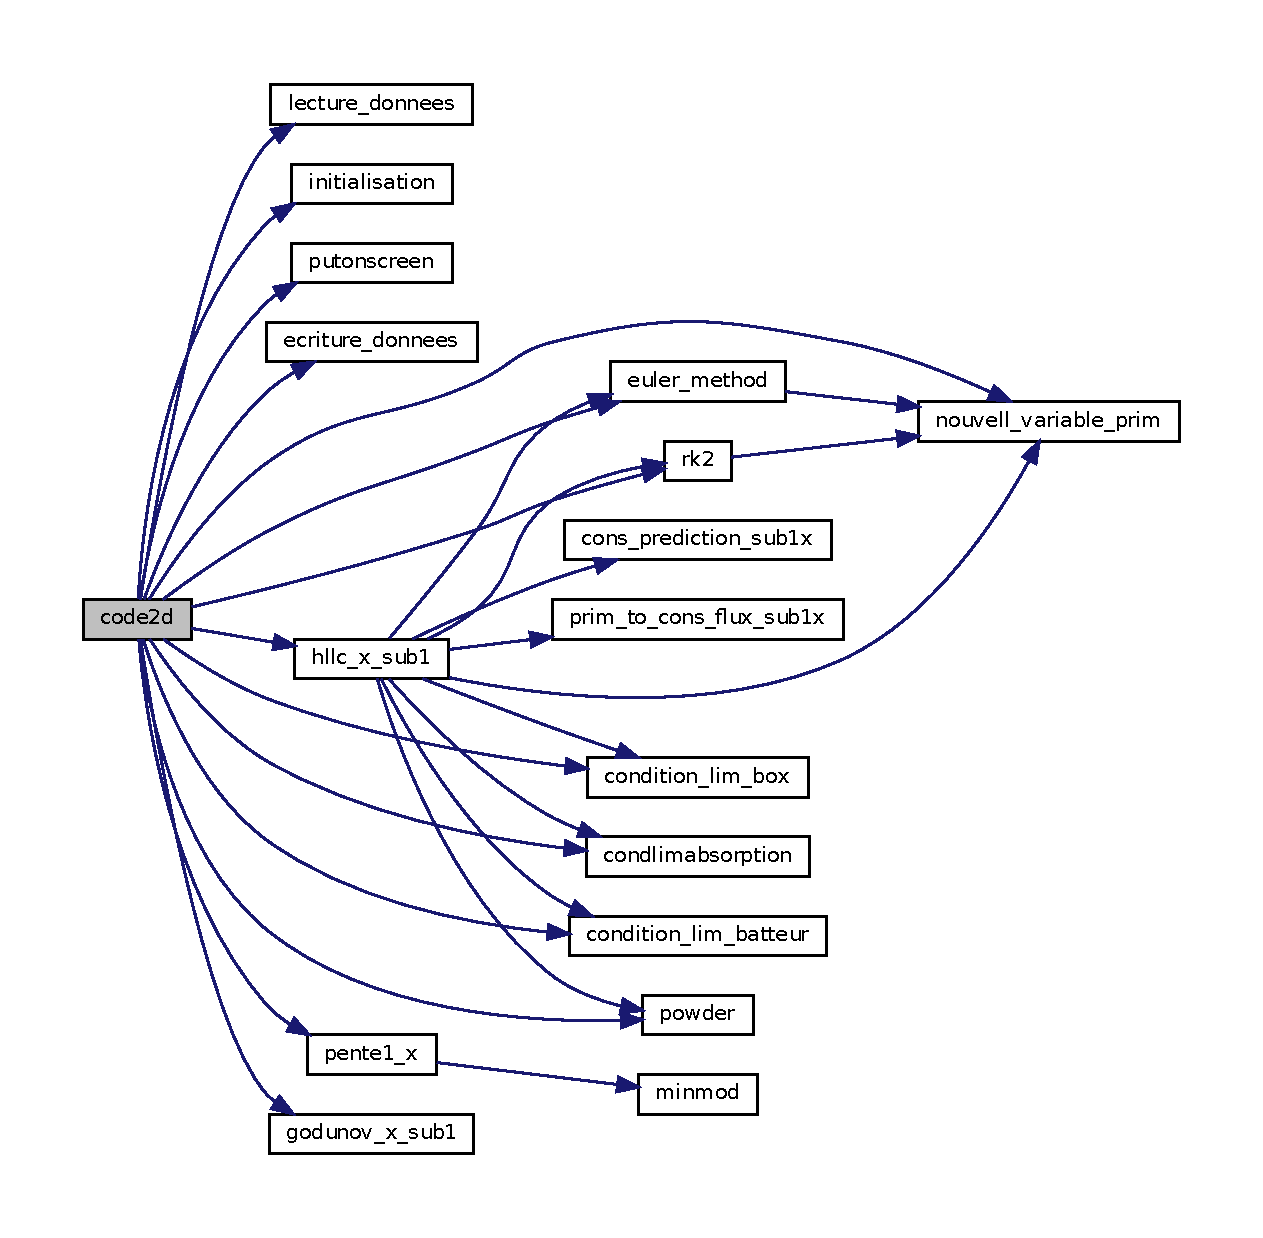
\includegraphics[width=350pt]{main1DOr2_8f90_a8712173bc20143ca5b1b8cbd782b563e_cgraph}
\end{center}
\end{figure}
\mbox{\Hypertarget{main1DOr2_8f90_ab89119a8e79210de76ccde93ce834633}\label{main1DOr2_8f90_ab89119a8e79210de76ccde93ce834633}} 
\index{main1\+D\+Or2.\+f90@{main1\+D\+Or2.\+f90}!condition\+\_\+lim\+\_\+batteur@{condition\+\_\+lim\+\_\+batteur}}
\index{condition\+\_\+lim\+\_\+batteur@{condition\+\_\+lim\+\_\+batteur}!main1\+D\+Or2.\+f90@{main1\+D\+Or2.\+f90}}
\subsubsection{\texorpdfstring{condition\+\_\+lim\+\_\+batteur()}{condition\_lim\_batteur()}}
{\footnotesize\ttfamily subroutine code2d\+::condition\+\_\+lim\+\_\+batteur (\begin{DoxyParamCaption}\item[{real (kind = dp), dimension(nv\+\_\+prim,0\+:nx+1)}]{Prim,  }\item[{real (kind = dp), dimension(0\+:nx+1)}]{Ein,  }\item[{real (kind = dp), dimension(0\+:nx+1)}]{Pression,  }\item[{real (kind = dp), dimension(0\+:nx+1)}]{S\+O\+U\+N\+D\+\_\+ax,  }\item[{real (kind = dp)}]{T\+I\+ME }\end{DoxyParamCaption})}

\mbox{\Hypertarget{main1DOr2_8f90_ae72ce7fe5060af7e7c56122d5232f6c3}\label{main1DOr2_8f90_ae72ce7fe5060af7e7c56122d5232f6c3}} 
\index{main1\+D\+Or2.\+f90@{main1\+D\+Or2.\+f90}!condition\+\_\+lim\+\_\+box@{condition\+\_\+lim\+\_\+box}}
\index{condition\+\_\+lim\+\_\+box@{condition\+\_\+lim\+\_\+box}!main1\+D\+Or2.\+f90@{main1\+D\+Or2.\+f90}}
\subsubsection{\texorpdfstring{condition\+\_\+lim\+\_\+box()}{condition\_lim\_box()}}
{\footnotesize\ttfamily subroutine code2d\+::condition\+\_\+lim\+\_\+box (\begin{DoxyParamCaption}\item[{real (kind = dp), dimension(nv\+\_\+prim,0\+:nx+1)}]{Prim,  }\item[{real (kind = dp), dimension(0\+:nx+1)}]{Ein,  }\item[{real (kind = dp), dimension(0\+:nx+1)}]{Pression,  }\item[{real (kind = dp), dimension(0\+:nx+1)}]{S\+O\+U\+N\+D\+\_\+ax }\end{DoxyParamCaption})}

\mbox{\Hypertarget{main1DOr2_8f90_abf21f0faeed0f3974f34fb740d77af75}\label{main1DOr2_8f90_abf21f0faeed0f3974f34fb740d77af75}} 
\index{main1\+D\+Or2.\+f90@{main1\+D\+Or2.\+f90}!condlimabsorption@{condlimabsorption}}
\index{condlimabsorption@{condlimabsorption}!main1\+D\+Or2.\+f90@{main1\+D\+Or2.\+f90}}
\subsubsection{\texorpdfstring{condlimabsorption()}{condlimabsorption()}}
{\footnotesize\ttfamily subroutine code2d\+::condlimabsorption (\begin{DoxyParamCaption}\item[{real (kind = dp), dimension(nv\+\_\+prim,0\+:nx+1)}]{Prim,  }\item[{real (kind = dp), dimension(0\+:nx+1)}]{Ein,  }\item[{real (kind = dp), dimension(0\+:nx+1)}]{Pression,  }\item[{real (kind = dp), dimension(0\+:nx+1)}]{S\+O\+U\+N\+D\+\_\+ax }\end{DoxyParamCaption})}

\mbox{\Hypertarget{main1DOr2_8f90_a41f5497b85eecbbc6af40d3959e67a3d}\label{main1DOr2_8f90_a41f5497b85eecbbc6af40d3959e67a3d}} 
\index{main1\+D\+Or2.\+f90@{main1\+D\+Or2.\+f90}!cons\+\_\+prediction\+\_\+sub1x@{cons\+\_\+prediction\+\_\+sub1x}}
\index{cons\+\_\+prediction\+\_\+sub1x@{cons\+\_\+prediction\+\_\+sub1x}!main1\+D\+Or2.\+f90@{main1\+D\+Or2.\+f90}}
\subsubsection{\texorpdfstring{cons\+\_\+prediction\+\_\+sub1x()}{cons\_prediction\_sub1x()}}
{\footnotesize\ttfamily subroutine code2d\+::cons\+\_\+prediction\+\_\+sub1x (\begin{DoxyParamCaption}\item[{real (kind = dp)}]{DX,  }\item[{real (kind = dp)}]{DT,  }\item[{real (kind = dp), dimension(nv\+\_\+prim,1\+:nx)}]{C\+O\+NS,  }\item[{real (kind = dp), dimension(nv\+\_\+prim,1\+:nx)}]{C\+O\+N\+S\+\_\+\+P\+R\+ED,  }\item[{real (kind = dp), dimension(nv\+\_\+prim,0\+:nx)}]{F\+L\+U\+X\+GG,  }\item[{real (kind = dp), dimension(nv\+\_\+prim,0\+:nx)}]{F\+L\+U\+X\+DD }\end{DoxyParamCaption})}

\mbox{\Hypertarget{main1DOr2_8f90_a47ac97fd58c2f9695ffff2ee98d498c1}\label{main1DOr2_8f90_a47ac97fd58c2f9695ffff2ee98d498c1}} 
\index{main1\+D\+Or2.\+f90@{main1\+D\+Or2.\+f90}!ecriture\+\_\+donnees@{ecriture\+\_\+donnees}}
\index{ecriture\+\_\+donnees@{ecriture\+\_\+donnees}!main1\+D\+Or2.\+f90@{main1\+D\+Or2.\+f90}}
\subsubsection{\texorpdfstring{ecriture\+\_\+donnees()}{ecriture\_donnees()}}
{\footnotesize\ttfamily subroutine code2d\+::ecriture\+\_\+donnees (\begin{DoxyParamCaption}\item[{real (kind = dp), dimension(1\+:nx)}]{X,  }\item[{real (kind = dp), dimension(nv\+\_\+prim,0\+:nx+1)}]{Prim,  }\item[{real (kind = dp), dimension(0\+:nx+1)}]{Ein,  }\item[{real (kind = dp), dimension(0\+:nx+1)}]{Pression,  }\item[{real (kind = dp)}]{time,  }\item[{real (kind = dp)}]{DX,  }\item[{real (kind = dp), dimension(1\+:nx)}]{U1,  }\item[{real (kind = dp)}]{Lx,  }\item[{real (kind = dp), dimension(1\+:nx)}]{Qaverage }\end{DoxyParamCaption})}

\mbox{\Hypertarget{main1DOr2_8f90_a61ef0ae28fb906748d601350a093a3fa}\label{main1DOr2_8f90_a61ef0ae28fb906748d601350a093a3fa}} 
\index{main1\+D\+Or2.\+f90@{main1\+D\+Or2.\+f90}!euler\+\_\+method@{euler\+\_\+method}}
\index{euler\+\_\+method@{euler\+\_\+method}!main1\+D\+Or2.\+f90@{main1\+D\+Or2.\+f90}}
\subsubsection{\texorpdfstring{euler\+\_\+method()}{euler\_method()}}
{\footnotesize\ttfamily subroutine code2d\+::euler\+\_\+method (\begin{DoxyParamCaption}\item[{real (kind = dp)}]{DT,  }\item[{real (kind = dp)}]{time,  }\item[{real (kind = dp), dimension(1\+:nx)}]{X,  }\item[{real (kind = dp), dimension(nv\+\_\+prim,1\+:nx)}]{C\+O\+NS,  }\item[{real (kind = dp), dimension(nv\+\_\+prim,0\+:nx+1)}]{Prim,  }\item[{real (kind = dp), dimension(0\+:nx+1)}]{Ein,  }\item[{real (kind = dp), dimension(0\+:nx+1)}]{S\+O\+U\+N\+D\+\_\+ax,  }\item[{real (kind = dp), dimension(0\+:nx+1)}]{Pression,  }\item[{integer}]{it,  }\item[{real (kind = dp), dimension(1\+:nx)}]{U1,  }\item[{real (kind = dp), dimension(1\+:nx)}]{Qaverage }\end{DoxyParamCaption})}

Here is the call graph for this function\+:
\nopagebreak
\begin{figure}[H]
\begin{center}
\leavevmode
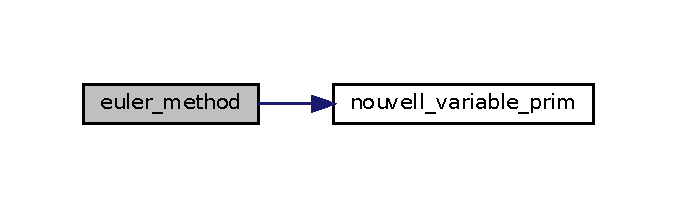
\includegraphics[width=325pt]{main1DOr2_8f90_a61ef0ae28fb906748d601350a093a3fa_cgraph}
\end{center}
\end{figure}
\mbox{\Hypertarget{main1DOr2_8f90_aec66a1d113ade1d60ad864482ea8e4cf}\label{main1DOr2_8f90_aec66a1d113ade1d60ad864482ea8e4cf}} 
\index{main1\+D\+Or2.\+f90@{main1\+D\+Or2.\+f90}!godunov\+\_\+x\+\_\+sub1@{godunov\+\_\+x\+\_\+sub1}}
\index{godunov\+\_\+x\+\_\+sub1@{godunov\+\_\+x\+\_\+sub1}!main1\+D\+Or2.\+f90@{main1\+D\+Or2.\+f90}}
\subsubsection{\texorpdfstring{godunov\+\_\+x\+\_\+sub1()}{godunov\_x\_sub1()}}
{\footnotesize\ttfamily subroutine code2d\+::godunov\+\_\+x\+\_\+sub1 (\begin{DoxyParamCaption}\item[{real(kind=dp), dimension(nv\+\_\+prim,1\+:nx)}]{cons,  }\item[{real(kind=dp), dimension(nv\+\_\+prim,0\+:nx)}]{flux,  }\item[{real(kind=dp)}]{dt,  }\item[{real(kind=dp)}]{dx }\end{DoxyParamCaption})}

\mbox{\Hypertarget{main1DOr2_8f90_a86edd837bdc9a015ebd8a46212fe70ab}\label{main1DOr2_8f90_a86edd837bdc9a015ebd8a46212fe70ab}} 
\index{main1\+D\+Or2.\+f90@{main1\+D\+Or2.\+f90}!hllc\+\_\+x\+\_\+sub1@{hllc\+\_\+x\+\_\+sub1}}
\index{hllc\+\_\+x\+\_\+sub1@{hllc\+\_\+x\+\_\+sub1}!main1\+D\+Or2.\+f90@{main1\+D\+Or2.\+f90}}
\subsubsection{\texorpdfstring{hllc\+\_\+x\+\_\+sub1()}{hllc\_x\_sub1()}}
{\footnotesize\ttfamily subroutine code2d\+::hllc\+\_\+x\+\_\+sub1 (\begin{DoxyParamCaption}\item[{real (kind = dp), dimension(nv\+\_\+prim,0\+:nx+1)}]{prim,  }\item[{real (kind = dp), dimension(nv\+\_\+prim,0\+:nx)}]{flux,  }\item[{real (kind = dp), dimension(nv\+\_\+prim,0\+:nx+1)}]{pente,  }\item[{real (kind = dp), dimension(nv\+\_\+prim,1\+:nx)}]{cons,  }\item[{integer}]{it,  }\item[{real(kind=dp)}]{dt }\end{DoxyParamCaption})}

Here is the call graph for this function\+:
\nopagebreak
\begin{figure}[H]
\begin{center}
\leavevmode
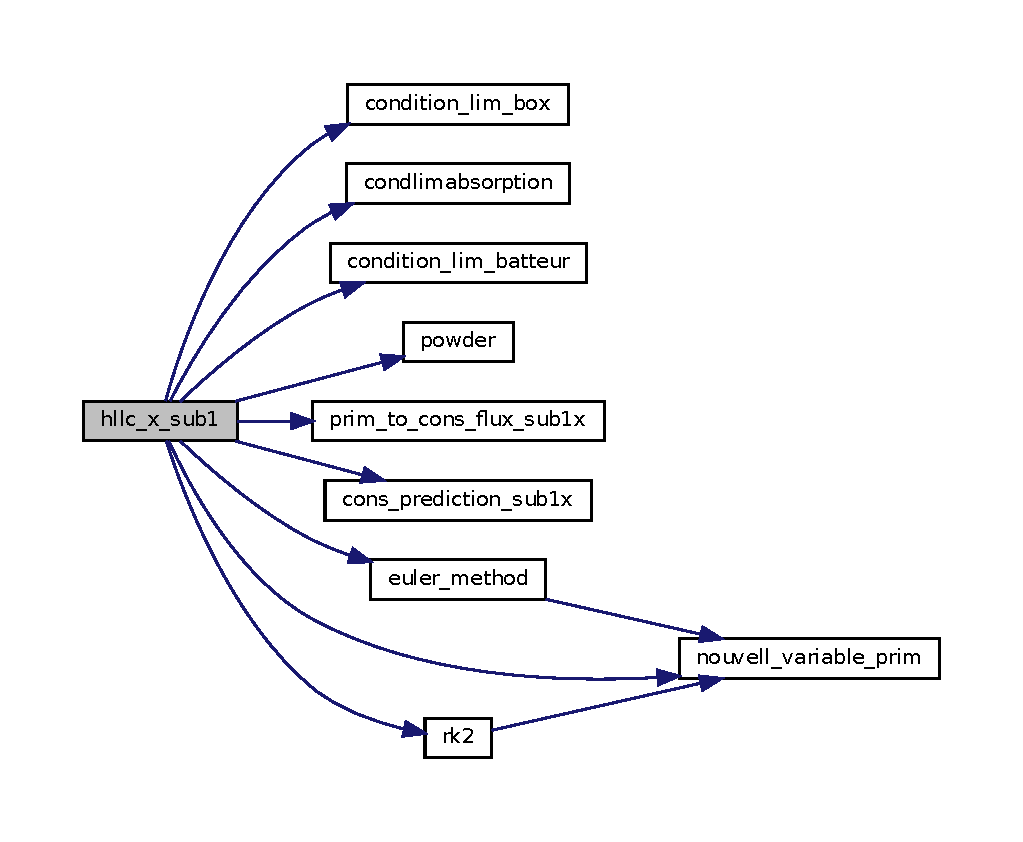
\includegraphics[width=350pt]{main1DOr2_8f90_a86edd837bdc9a015ebd8a46212fe70ab_cgraph}
\end{center}
\end{figure}
\mbox{\Hypertarget{main1DOr2_8f90_a2ab28d5afcb8110dd4d60685348cb3d3}\label{main1DOr2_8f90_a2ab28d5afcb8110dd4d60685348cb3d3}} 
\index{main1\+D\+Or2.\+f90@{main1\+D\+Or2.\+f90}!initialisation@{initialisation}}
\index{initialisation@{initialisation}!main1\+D\+Or2.\+f90@{main1\+D\+Or2.\+f90}}
\subsubsection{\texorpdfstring{initialisation()}{initialisation()}}
{\footnotesize\ttfamily subroutine code2d\+::initialisation (\begin{DoxyParamCaption}\item[{real (kind = dp)}]{DX,  }\item[{real (kind = dp), dimension(1\+:nx)}]{X,  }\item[{real (kind = dp), dimension(nv\+\_\+prim, 0\+:nx+1)}]{Prim,  }\item[{real (kind = dp), dimension(0\+:nx+1)}]{S\+O\+U\+N\+D\+\_\+ax,  }\item[{real (kind = dp), dimension(0\+:nx+1)}]{Ein,  }\item[{real (kind = dp), dimension(nv\+\_\+prim,1\+:nx)}]{C\+O\+NS,  }\item[{real (kind = dp), dimension(0\+:nx+1)}]{Pression,  }\item[{real (kind = dp)}]{Lx }\end{DoxyParamCaption})}

\mbox{\Hypertarget{main1DOr2_8f90_a62516b42ea4fb4c0918eb7e43982d4a8}\label{main1DOr2_8f90_a62516b42ea4fb4c0918eb7e43982d4a8}} 
\index{main1\+D\+Or2.\+f90@{main1\+D\+Or2.\+f90}!lecture\+\_\+donnees@{lecture\+\_\+donnees}}
\index{lecture\+\_\+donnees@{lecture\+\_\+donnees}!main1\+D\+Or2.\+f90@{main1\+D\+Or2.\+f90}}
\subsubsection{\texorpdfstring{lecture\+\_\+donnees()}{lecture\_donnees()}}
{\footnotesize\ttfamily subroutine code2d\+::lecture\+\_\+donnees (\begin{DoxyParamCaption}\item[{real (kind = dp)}]{Lx }\end{DoxyParamCaption})}

\mbox{\Hypertarget{main1DOr2_8f90_a782814db45b1ac79c2d169964b28fd07}\label{main1DOr2_8f90_a782814db45b1ac79c2d169964b28fd07}} 
\index{main1\+D\+Or2.\+f90@{main1\+D\+Or2.\+f90}!minmod@{minmod}}
\index{minmod@{minmod}!main1\+D\+Or2.\+f90@{main1\+D\+Or2.\+f90}}
\subsubsection{\texorpdfstring{minmod()}{minmod()}}
{\footnotesize\ttfamily subroutine code2d\+::minmod (\begin{DoxyParamCaption}\item[{real(kind=dp)}]{s1,  }\item[{real(kind=dp)}]{s2,  }\item[{real(kind=dp)}]{slim }\end{DoxyParamCaption})}

\mbox{\Hypertarget{main1DOr2_8f90_aa208014933dc346cd26290f44b072d66}\label{main1DOr2_8f90_aa208014933dc346cd26290f44b072d66}} 
\index{main1\+D\+Or2.\+f90@{main1\+D\+Or2.\+f90}!nouvell\+\_\+variable\+\_\+prim@{nouvell\+\_\+variable\+\_\+prim}}
\index{nouvell\+\_\+variable\+\_\+prim@{nouvell\+\_\+variable\+\_\+prim}!main1\+D\+Or2.\+f90@{main1\+D\+Or2.\+f90}}
\subsubsection{\texorpdfstring{nouvell\+\_\+variable\+\_\+prim()}{nouvell\_variable\_prim()}}
{\footnotesize\ttfamily subroutine code2d\+::nouvell\+\_\+variable\+\_\+prim (\begin{DoxyParamCaption}\item[{real (kind = dp), dimension(nv\+\_\+prim,0\+:nx+1)}]{Prim,  }\item[{real (kind = dp), dimension(0\+:nx+1)}]{Ein,  }\item[{real (kind = dp), dimension(0\+:nx+1)}]{S\+O\+U\+N\+D\+\_\+ax,  }\item[{real (kind = dp), dimension(nv\+\_\+prim,1\+:nx)}]{C\+O\+NS,  }\item[{real (kind = dp), dimension(0\+:nx+1)}]{Pression,  }\item[{integer}]{it }\end{DoxyParamCaption})}

\mbox{\Hypertarget{main1DOr2_8f90_ab1369821f897b816d4e9a8f6740ea693}\label{main1DOr2_8f90_ab1369821f897b816d4e9a8f6740ea693}} 
\index{main1\+D\+Or2.\+f90@{main1\+D\+Or2.\+f90}!pente1\+\_\+x@{pente1\+\_\+x}}
\index{pente1\+\_\+x@{pente1\+\_\+x}!main1\+D\+Or2.\+f90@{main1\+D\+Or2.\+f90}}
\subsubsection{\texorpdfstring{pente1\+\_\+x()}{pente1\_x()}}
{\footnotesize\ttfamily subroutine code2d\+::pente1\+\_\+x (\begin{DoxyParamCaption}\item[{real (kind = dp), dimension(nv\+\_\+prim,0\+:nx+1)}]{Prim,  }\item[{real (kind = dp), dimension(nv\+\_\+prim,0\+:nx+1)}]{P\+E\+N\+TE }\end{DoxyParamCaption})}

Here is the call graph for this function\+:
\nopagebreak
\begin{figure}[H]
\begin{center}
\leavevmode
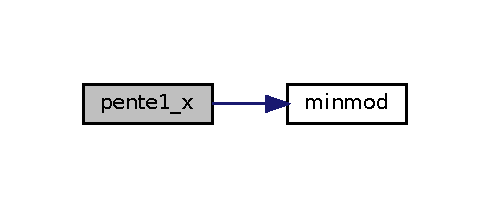
\includegraphics[width=235pt]{main1DOr2_8f90_ab1369821f897b816d4e9a8f6740ea693_cgraph}
\end{center}
\end{figure}
\mbox{\Hypertarget{main1DOr2_8f90_a9a3d7ad4173d691f4f090f6c4c4e05b3}\label{main1DOr2_8f90_a9a3d7ad4173d691f4f090f6c4c4e05b3}} 
\index{main1\+D\+Or2.\+f90@{main1\+D\+Or2.\+f90}!powder@{powder}}
\index{powder@{powder}!main1\+D\+Or2.\+f90@{main1\+D\+Or2.\+f90}}
\subsubsection{\texorpdfstring{powder()}{powder()}}
{\footnotesize\ttfamily subroutine code2d\+::powder (\begin{DoxyParamCaption}\item[{real (kind = dp), dimension(nv\+\_\+prim,0\+:nx+1)}]{Prim,  }\item[{real (kind = dp), dimension(0\+:nx+1)}]{Ein,  }\item[{real (kind = dp), dimension(0\+:nx+1)}]{Pression,  }\item[{real (kind = dp), dimension(0\+:nx+1)}]{S\+O\+U\+N\+D\+\_\+ax }\end{DoxyParamCaption})}

\mbox{\Hypertarget{main1DOr2_8f90_a1054c20993438d4f9ef5cc742a3245b4}\label{main1DOr2_8f90_a1054c20993438d4f9ef5cc742a3245b4}} 
\index{main1\+D\+Or2.\+f90@{main1\+D\+Or2.\+f90}!prim\+\_\+to\+\_\+cons\+\_\+flux\+\_\+sub1x@{prim\+\_\+to\+\_\+cons\+\_\+flux\+\_\+sub1x}}
\index{prim\+\_\+to\+\_\+cons\+\_\+flux\+\_\+sub1x@{prim\+\_\+to\+\_\+cons\+\_\+flux\+\_\+sub1x}!main1\+D\+Or2.\+f90@{main1\+D\+Or2.\+f90}}
\subsubsection{\texorpdfstring{prim\+\_\+to\+\_\+cons\+\_\+flux\+\_\+sub1x()}{prim\_to\_cons\_flux\_sub1x()}}
{\footnotesize\ttfamily subroutine code2d\+::prim\+\_\+to\+\_\+cons\+\_\+flux\+\_\+sub1x (\begin{DoxyParamCaption}\item[{real (kind = dp), dimension(nv\+\_\+prim,0\+:nx+1)}]{Prim,  }\item[{real (kind = dp), dimension(0\+:nx+1)}]{Ein,  }\item[{real (kind = dp), dimension(0\+:nx+1)}]{Pression,  }\item[{real (kind = dp), dimension(nv\+\_\+prim,1\+:nx)}]{C\+O\+NS,  }\item[{real (kind = dp), dimension(nv\+\_\+prim,0\+:nx)}]{F\+L\+UX }\end{DoxyParamCaption})}

\mbox{\Hypertarget{main1DOr2_8f90_a8a5b072c001df1496416cc96562c9916}\label{main1DOr2_8f90_a8a5b072c001df1496416cc96562c9916}} 
\index{main1\+D\+Or2.\+f90@{main1\+D\+Or2.\+f90}!putonscreen@{putonscreen}}
\index{putonscreen@{putonscreen}!main1\+D\+Or2.\+f90@{main1\+D\+Or2.\+f90}}
\subsubsection{\texorpdfstring{putonscreen()}{putonscreen()}}
{\footnotesize\ttfamily subroutine code2d\+::putonscreen (\begin{DoxyParamCaption}{ }\end{DoxyParamCaption})}

\mbox{\Hypertarget{main1DOr2_8f90_abf018793b221c901580957ed90346b9d}\label{main1DOr2_8f90_abf018793b221c901580957ed90346b9d}} 
\index{main1\+D\+Or2.\+f90@{main1\+D\+Or2.\+f90}!rk2@{rk2}}
\index{rk2@{rk2}!main1\+D\+Or2.\+f90@{main1\+D\+Or2.\+f90}}
\subsubsection{\texorpdfstring{rk2()}{rk2()}}
{\footnotesize\ttfamily subroutine code2d\+::rk2 (\begin{DoxyParamCaption}\item[{real (kind = dp)}]{DT,  }\item[{real (kind = dp), dimension(nv\+\_\+prim,1\+:nx)}]{C\+O\+NS,  }\item[{real (kind = dp), dimension(nv\+\_\+prim,0\+:nx+1)}]{Prim,  }\item[{real (kind = dp), dimension(0\+:nx+1)}]{Ein,  }\item[{real (kind = dp), dimension(0\+:nx+1)}]{S\+O\+U\+N\+D\+\_\+ax,  }\item[{real (kind = dp), dimension(0\+:nx+1)}]{Pression,  }\item[{integer}]{it,  }\item[{real (kind = dp), dimension(1\+:nx)}]{U1 }\end{DoxyParamCaption})}

Here is the call graph for this function\+:
\nopagebreak
\begin{figure}[H]
\begin{center}
\leavevmode
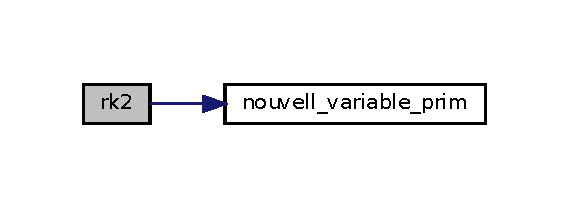
\includegraphics[width=273pt]{main1DOr2_8f90_abf018793b221c901580957ed90346b9d_cgraph}
\end{center}
\end{figure}
\mbox{\Hypertarget{main1DOr2_8f90_a1584e44687072629ab256df4b8fe6537}\label{main1DOr2_8f90_a1584e44687072629ab256df4b8fe6537}} 
\index{main1\+D\+Or2.\+f90@{main1\+D\+Or2.\+f90}!superbee@{superbee}}
\index{superbee@{superbee}!main1\+D\+Or2.\+f90@{main1\+D\+Or2.\+f90}}
\subsubsection{\texorpdfstring{superbee()}{superbee()}}
{\footnotesize\ttfamily subroutine code2d\+::superbee (\begin{DoxyParamCaption}\item[{real(kind=dp)}]{s1,  }\item[{real(kind=dp)}]{s2,  }\item[{real(kind=dp)}]{slim }\end{DoxyParamCaption})}

\mbox{\Hypertarget{main1DOr2_8f90_ac6b2b51b381114cb3bc7fa9abc69dee7}\label{main1DOr2_8f90_ac6b2b51b381114cb3bc7fa9abc69dee7}} 
\index{main1\+D\+Or2.\+f90@{main1\+D\+Or2.\+f90}!valbada@{valbada}}
\index{valbada@{valbada}!main1\+D\+Or2.\+f90@{main1\+D\+Or2.\+f90}}
\subsubsection{\texorpdfstring{valbada()}{valbada()}}
{\footnotesize\ttfamily subroutine code2d\+::valbada (\begin{DoxyParamCaption}\item[{real(kind=dp)}]{s1,  }\item[{real(kind=dp)}]{s2,  }\item[{real(kind=dp)}]{slim }\end{DoxyParamCaption})}

\mbox{\Hypertarget{main1DOr2_8f90_af50a25d9d5f073c1347e643d589770ac}\label{main1DOr2_8f90_af50a25d9d5f073c1347e643d589770ac}} 
\index{main1\+D\+Or2.\+f90@{main1\+D\+Or2.\+f90}!vleer@{vleer}}
\index{vleer@{vleer}!main1\+D\+Or2.\+f90@{main1\+D\+Or2.\+f90}}
\subsubsection{\texorpdfstring{vleer()}{vleer()}}
{\footnotesize\ttfamily subroutine code2d\+::vleer (\begin{DoxyParamCaption}\item[{real(kind=dp)}]{s1,  }\item[{real(kind=dp)}]{s2,  }\item[{real(kind=dp)}]{slim }\end{DoxyParamCaption})}

\mbox{\Hypertarget{main1DOr2_8f90_a236c2f231e6eabfc3ddff4bc2f56bb99}\label{main1DOr2_8f90_a236c2f231e6eabfc3ddff4bc2f56bb99}} 
\index{main1\+D\+Or2.\+f90@{main1\+D\+Or2.\+f90}!vmc@{vmc}}
\index{vmc@{vmc}!main1\+D\+Or2.\+f90@{main1\+D\+Or2.\+f90}}
\subsubsection{\texorpdfstring{vmc()}{vmc()}}
{\footnotesize\ttfamily subroutine code2d\+::vmc (\begin{DoxyParamCaption}\item[{real(kind=dp)}]{s1,  }\item[{real(kind=dp)}]{s2,  }\item[{real(kind=dp)}]{slim }\end{DoxyParamCaption})}


\hypertarget{main2Dv1_01_07copy_08_8f90}{}\section{src/main2\+Dv1 (copy).f90 File Reference}
\label{main2Dv1_01_07copy_08_8f90}\index{src/main2\+Dv1 (copy).\+f90@{src/main2\+Dv1 (copy).\+f90}}
\subsection*{Modules}
\begin{DoxyCompactItemize}
\item 
module \mbox{\hyperlink{namespaceprecisions}{precisions}}
\item 
module \mbox{\hyperlink{namespaceglobalparam}{globalparam}}
\item 
module \mbox{\hyperlink{namespacemodeleinterface}{modeleinterface}}
\end{DoxyCompactItemize}
\subsection*{Functions/\+Subroutines}
\begin{DoxyCompactItemize}
\item 
real(kind=dp) function \mbox{\hyperlink{namespacemodeleinterface_a4d0b51322903b5a095f04aaafb1a8c5f}{modeleinterface\+::internalen}} (h, p11, p22)
\item 
real(kind=dp) function \mbox{\hyperlink{namespacemodeleinterface_ad34088de8c0162343994153e8f34921e}{modeleinterface\+::press}} (h, p11)
\item 
real(kind=dp) function \mbox{\hyperlink{namespacemodeleinterface_a1505c575aa44b45a8509fe827f28bc8d}{modeleinterface\+::sound\+\_\+a\+\_\+x}} (h, p11)
\item 
real(kind=dp) function \mbox{\hyperlink{namespacemodeleinterface_aea42339ec55b6d0e7333dcd4c2d6041f}{modeleinterface\+::sound\+\_\+a\+\_\+y}} (h, p22)
\item 
real(kind=dp) function \mbox{\hyperlink{namespacemodeleinterface_aa422a9d23665a7fa175a3458f15d6be2}{modeleinterface\+::sound\+\_\+b\+\_\+x}} (p11)
\item 
real(kind=dp) function \mbox{\hyperlink{namespacemodeleinterface_ae6539d207be975bdb5b8c45826062a30}{modeleinterface\+::sound\+\_\+b\+\_\+y}} (p22)
\item 
program \mbox{\hyperlink{main2Dv1_01_07copy_08_8f90_a8712173bc20143ca5b1b8cbd782b563e}{code2d}}
\item 
subroutine \mbox{\hyperlink{main2Dv1_01_07copy_08_8f90_ad651365c868e762b033239f23065b179}{hllc\+\_\+x\+\_\+sub1}} (prim, flux)
\item 
subroutine \mbox{\hyperlink{main2Dv1_01_07copy_08_8f90_a542b368221e3c5b6eed538ddc6538ca5}{hllc\+\_\+x\+\_\+sub2}} (prim, flux)
\item 
subroutine \mbox{\hyperlink{main2Dv1_01_07copy_08_8f90_aec66a1d113ade1d60ad864482ea8e4cf}{godunov\+\_\+x\+\_\+sub1}} (cons, flux, dt, dx)
\item 
subroutine \mbox{\hyperlink{main2Dv1_01_07copy_08_8f90_a95998c355563e1e58114aea99de5433b}{godunov\+\_\+x\+\_\+sub2}} (cons, flux, dt, dx)
\item 
subroutine \mbox{\hyperlink{main2Dv1_01_07copy_08_8f90_a3abf545225182ebde80c72121d2de6f2}{hllc\+\_\+y\+\_\+sub1}} (prim, flux)
\item 
subroutine \mbox{\hyperlink{main2Dv1_01_07copy_08_8f90_a66b4ae2bdd9b70fca9079c3827fa8c30}{hllc\+\_\+y\+\_\+sub2}} (prim, flux)
\item 
subroutine \mbox{\hyperlink{main2Dv1_01_07copy_08_8f90_a99b7b2764471880074ec2cb4448c3232}{godunov\+\_\+y\+\_\+sub1}} (cons, flux, dt, dx)
\item 
subroutine \mbox{\hyperlink{main2Dv1_01_07copy_08_8f90_af2bc178b3e046a285b7e624ecb7246b8}{godunov\+\_\+y\+\_\+sub2}} (cons, flux, dt, dx)
\item 
subroutine \mbox{\hyperlink{main2Dv1_01_07copy_08_8f90_a8a5b072c001df1496416cc96562c9916}{putonscreen}} ()
\item 
subroutine \mbox{\hyperlink{main2Dv1_01_07copy_08_8f90_aff02bfa8466e376e08fed7a99aae4039}{ecriture\+\_\+donnees}} (X, Y, Lx, Prim, Ein, Pression, time, DX, DY)
\item 
subroutine \mbox{\hyperlink{main2Dv1_01_07copy_08_8f90_a7e06ba833aef7743b6a2f1be79f4bc2e}{lecture\+\_\+donnees}} (Lx, Ly)
\item 
subroutine \mbox{\hyperlink{main2Dv1_01_07copy_08_8f90_afb1c4be5a540eb38b6217aa886b964a5}{initialisation}} (DX, DY, X, Y, Prim, S\+O\+U\+N\+D\+\_\+ax, S\+O\+U\+N\+D\+\_\+bx, S\+O\+U\+N\+D\+\_\+ay, S\+O\+U\+N\+D\+\_\+by, Ein, C\+O\+NS, Pression, Lx)
\item 
subroutine \mbox{\hyperlink{main2Dv1_01_07copy_08_8f90_a7e8756401e9774b000709214edc41a76}{nouvell\+\_\+variable\+\_\+prim}} (Prim, Ein, S\+O\+U\+N\+D\+\_\+ax, S\+O\+U\+N\+D\+\_\+bx, S\+O\+U\+N\+D\+\_\+ay, S\+O\+U\+N\+D\+\_\+by, C\+O\+NS, Pression, it)
\item 
subroutine \mbox{\hyperlink{main2Dv1_01_07copy_08_8f90_a2e4131a2a733710c33c03656b6a7fb34}{condition\+\_\+lim\+\_\+box}} (Prim, Ein, Pression, S\+O\+U\+N\+D\+\_\+ax, S\+O\+U\+N\+D\+\_\+bx, S\+O\+U\+N\+D\+\_\+ay, S\+O\+U\+N\+D\+\_\+by)
\item 
subroutine \mbox{\hyperlink{main2Dv1_01_07copy_08_8f90_a4fa8d6d2b6084471f67e67e44694e3a7}{condlimabsorption}} (Prim, Ein, Pression, S\+O\+U\+N\+D\+\_\+ax, S\+O\+U\+N\+D\+\_\+bx, S\+O\+U\+N\+D\+\_\+ay, S\+O\+U\+N\+D\+\_\+by)
\item 
subroutine \mbox{\hyperlink{main2Dv1_01_07copy_08_8f90_ae64974281df2d6f2222187665fd79e38}{condition\+\_\+lim\+\_\+batteur}} (Prim, Ein, Pression, S\+O\+U\+N\+D\+\_\+ax, S\+O\+U\+N\+D\+\_\+bx, S\+O\+U\+N\+D\+\_\+ay, S\+O\+U\+N\+D\+\_\+by, T\+I\+ME)
\item 
subroutine \mbox{\hyperlink{main2Dv1_01_07copy_08_8f90_a1874243fd0ebdb9c1e1cd78468b4cfac}{euler\+\_\+method}} (DT, time, Lx, X, Y, C\+O\+NS, Prim, Ein, S\+O\+U\+N\+D\+\_\+ax, S\+O\+U\+N\+D\+\_\+bx, S\+O\+U\+N\+D\+\_\+ay, S\+O\+U\+N\+D\+\_\+by, Pression, it)
\end{DoxyCompactItemize}
\subsection*{Variables}
\begin{DoxyCompactItemize}
\item 
integer \mbox{\hyperlink{namespaceglobalparam_ae3e17c94b4a693ce99dc99ca85e3aba5}{globalparam\+::ny}}
\item 
integer \mbox{\hyperlink{namespaceglobalparam_a980a183375fbe21d1ba02b3611dcc94d}{globalparam\+::v\+\_\+pv}}
\item 
integer \mbox{\hyperlink{namespaceglobalparam_a454092edac459f96bb9045ced3f632bd}{globalparam\+::p11\+\_\+pv}}
\item 
integer \mbox{\hyperlink{namespaceglobalparam_a9d0f6eb467ec66a6825d64e743f0fc36}{globalparam\+::p12\+\_\+pv}}
\item 
integer \mbox{\hyperlink{namespaceglobalparam_a1c0b88f532e0bb8c21c4aa92a92405ca}{globalparam\+::p22\+\_\+pv}}
\item 
real(kind=dp) \mbox{\hyperlink{namespaceglobalparam_a6192d97c147b8b0f5ebda79933dd6f16}{globalparam\+::y0}}
\item 
real(kind=dp) \mbox{\hyperlink{namespaceglobalparam_afcf85dea7c5d650ef77d480eb6d2a614}{globalparam\+::lambda}}
\item 
real(kind=dp) \mbox{\hyperlink{namespaceglobalparam_a22c2013f9cb1fb03d79e99fc038d55d1}{globalparam\+::gamma}}
\item 
real(kind=dp) \mbox{\hyperlink{namespaceglobalparam_a71ed33aead9f8bd6716557281b189e3c}{globalparam\+::beta}}
\end{DoxyCompactItemize}


\subsection{Function/\+Subroutine Documentation}
\mbox{\Hypertarget{main2Dv1_01_07copy_08_8f90_a8712173bc20143ca5b1b8cbd782b563e}\label{main2Dv1_01_07copy_08_8f90_a8712173bc20143ca5b1b8cbd782b563e}} 
\index{main2\+Dv1 (copy).\+f90@{main2\+Dv1 (copy).\+f90}!code2d@{code2d}}
\index{code2d@{code2d}!main2\+Dv1 (copy).\+f90@{main2\+Dv1 (copy).\+f90}}
\subsubsection{\texorpdfstring{code2d()}{code2d()}}
{\footnotesize\ttfamily program code2d (\begin{DoxyParamCaption}{ }\end{DoxyParamCaption})}

Here is the call graph for this function\+:
\nopagebreak
\begin{figure}[H]
\begin{center}
\leavevmode
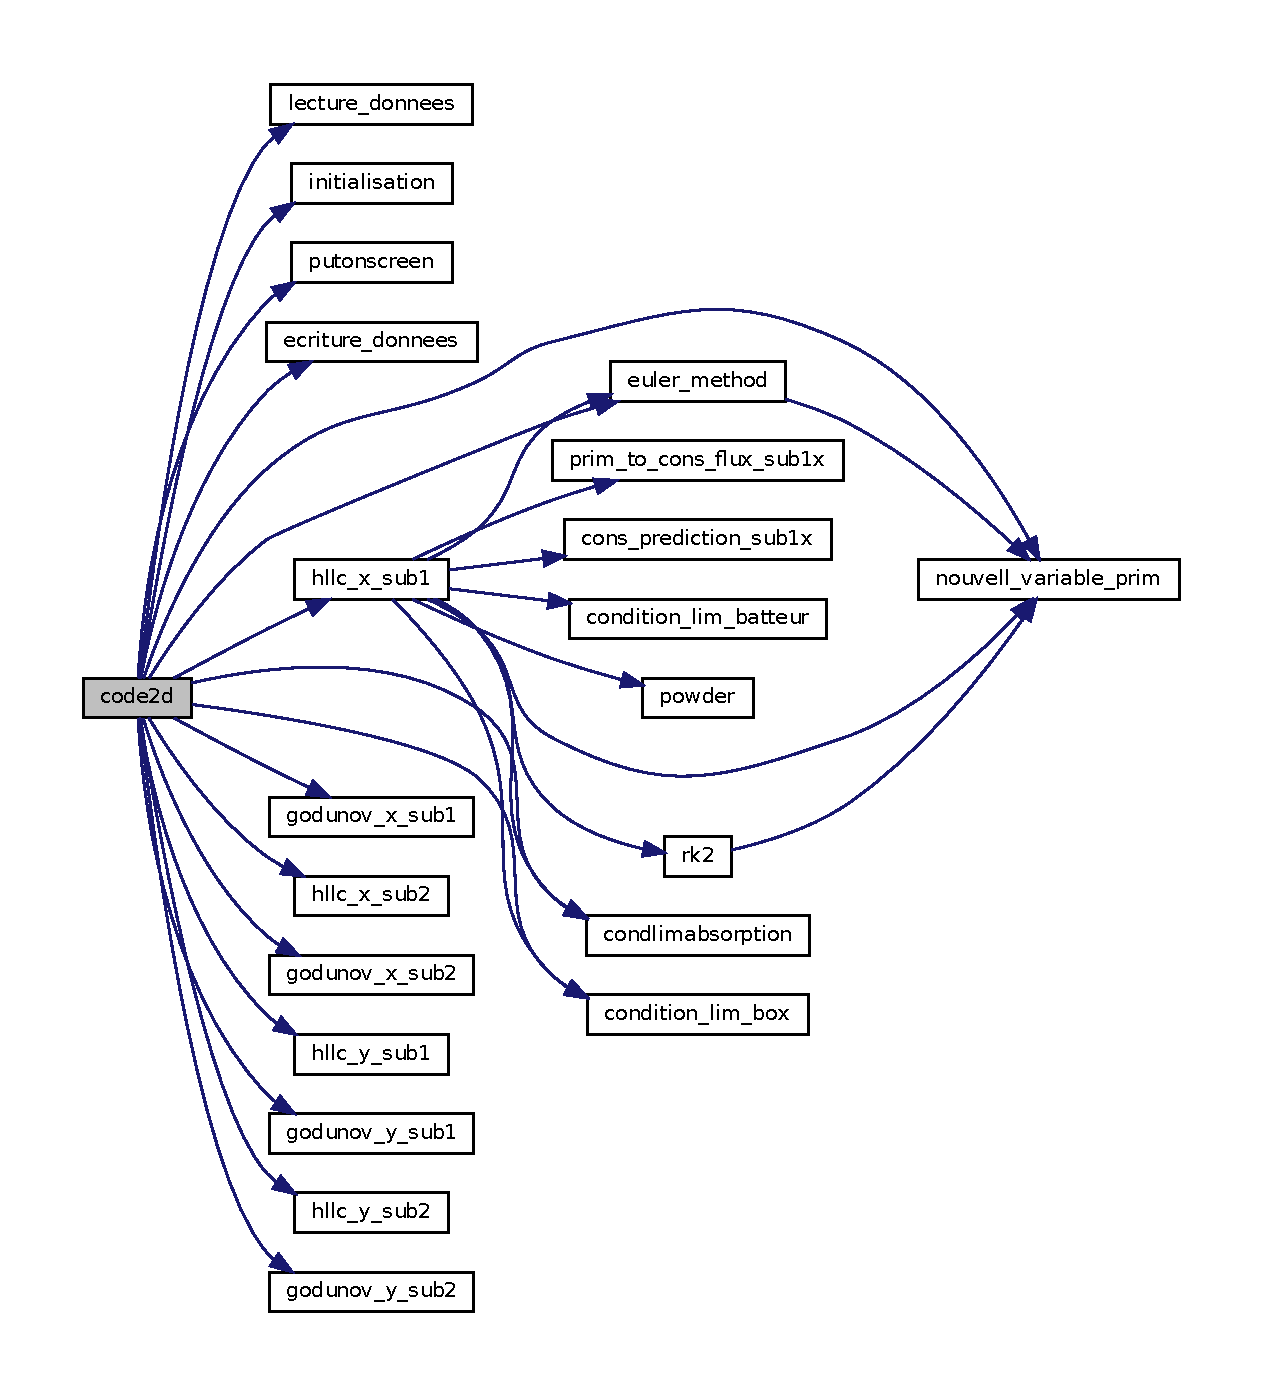
\includegraphics[width=350pt]{main2Dv1_01_07copy_08_8f90_a8712173bc20143ca5b1b8cbd782b563e_cgraph}
\end{center}
\end{figure}
\mbox{\Hypertarget{main2Dv1_01_07copy_08_8f90_ae64974281df2d6f2222187665fd79e38}\label{main2Dv1_01_07copy_08_8f90_ae64974281df2d6f2222187665fd79e38}} 
\index{main2\+Dv1 (copy).\+f90@{main2\+Dv1 (copy).\+f90}!condition\+\_\+lim\+\_\+batteur@{condition\+\_\+lim\+\_\+batteur}}
\index{condition\+\_\+lim\+\_\+batteur@{condition\+\_\+lim\+\_\+batteur}!main2\+Dv1 (copy).\+f90@{main2\+Dv1 (copy).\+f90}}
\subsubsection{\texorpdfstring{condition\+\_\+lim\+\_\+batteur()}{condition\_lim\_batteur()}}
{\footnotesize\ttfamily subroutine code2d\+::condition\+\_\+lim\+\_\+batteur (\begin{DoxyParamCaption}\item[{real (kind = dp), dimension(7,0\+:nx+1,0\+:ny+1)}]{Prim,  }\item[{real (kind = dp), dimension(0\+:nx+1,0\+:ny+1)}]{Ein,  }\item[{real (kind = dp), dimension(0\+:nx+1,0\+:ny+1)}]{Pression,  }\item[{real (kind = dp), dimension(0\+:nx+1,0\+:ny+1)}]{S\+O\+U\+N\+D\+\_\+ax,  }\item[{real (kind = dp), dimension(0\+:nx+1,0\+:ny+1)}]{S\+O\+U\+N\+D\+\_\+bx,  }\item[{real (kind = dp), dimension(0\+:nx+1,0\+:ny+1)}]{S\+O\+U\+N\+D\+\_\+ay,  }\item[{real (kind = dp), dimension(0\+:nx+1,0\+:ny+1)}]{S\+O\+U\+N\+D\+\_\+by,  }\item[{real (kind = dp)}]{T\+I\+ME }\end{DoxyParamCaption})}

\mbox{\Hypertarget{main2Dv1_01_07copy_08_8f90_a2e4131a2a733710c33c03656b6a7fb34}\label{main2Dv1_01_07copy_08_8f90_a2e4131a2a733710c33c03656b6a7fb34}} 
\index{main2\+Dv1 (copy).\+f90@{main2\+Dv1 (copy).\+f90}!condition\+\_\+lim\+\_\+box@{condition\+\_\+lim\+\_\+box}}
\index{condition\+\_\+lim\+\_\+box@{condition\+\_\+lim\+\_\+box}!main2\+Dv1 (copy).\+f90@{main2\+Dv1 (copy).\+f90}}
\subsubsection{\texorpdfstring{condition\+\_\+lim\+\_\+box()}{condition\_lim\_box()}}
{\footnotesize\ttfamily subroutine code2d\+::condition\+\_\+lim\+\_\+box (\begin{DoxyParamCaption}\item[{real (kind = dp), dimension(7,0\+:nx+1,0\+:ny+1)}]{Prim,  }\item[{real (kind = dp), dimension(0\+:nx+1,0\+:ny+1)}]{Ein,  }\item[{real (kind = dp), dimension(0\+:nx+1,0\+:ny+1)}]{Pression,  }\item[{real (kind = dp), dimension(0\+:nx+1,0\+:ny+1)}]{S\+O\+U\+N\+D\+\_\+ax,  }\item[{real (kind = dp), dimension(0\+:nx+1,0\+:ny+1)}]{S\+O\+U\+N\+D\+\_\+bx,  }\item[{real (kind = dp), dimension(0\+:nx+1,0\+:ny+1)}]{S\+O\+U\+N\+D\+\_\+ay,  }\item[{real (kind = dp), dimension(0\+:nx+1,0\+:ny+1)}]{S\+O\+U\+N\+D\+\_\+by }\end{DoxyParamCaption})}

\mbox{\Hypertarget{main2Dv1_01_07copy_08_8f90_a4fa8d6d2b6084471f67e67e44694e3a7}\label{main2Dv1_01_07copy_08_8f90_a4fa8d6d2b6084471f67e67e44694e3a7}} 
\index{main2\+Dv1 (copy).\+f90@{main2\+Dv1 (copy).\+f90}!condlimabsorption@{condlimabsorption}}
\index{condlimabsorption@{condlimabsorption}!main2\+Dv1 (copy).\+f90@{main2\+Dv1 (copy).\+f90}}
\subsubsection{\texorpdfstring{condlimabsorption()}{condlimabsorption()}}
{\footnotesize\ttfamily subroutine code2d\+::condlimabsorption (\begin{DoxyParamCaption}\item[{real (kind = dp), dimension(nv\+\_\+prim,0\+:nx+1,0\+:ny+1)}]{Prim,  }\item[{real (kind = dp), dimension(0\+:nx+1,0\+:ny+1)}]{Ein,  }\item[{real (kind = dp), dimension(0\+:nx+1,0\+:ny+1)}]{Pression,  }\item[{real (kind = dp), dimension(0\+:nx+1,0\+:ny+1)}]{S\+O\+U\+N\+D\+\_\+ax,  }\item[{real (kind = dp), dimension(0\+:nx+1,0\+:ny+1)}]{S\+O\+U\+N\+D\+\_\+bx,  }\item[{real (kind = dp), dimension(0\+:nx+1,0\+:ny+1)}]{S\+O\+U\+N\+D\+\_\+ay,  }\item[{real (kind = dp), dimension(0\+:nx+1,0\+:ny+1)}]{S\+O\+U\+N\+D\+\_\+by }\end{DoxyParamCaption})}

\mbox{\Hypertarget{main2Dv1_01_07copy_08_8f90_aff02bfa8466e376e08fed7a99aae4039}\label{main2Dv1_01_07copy_08_8f90_aff02bfa8466e376e08fed7a99aae4039}} 
\index{main2\+Dv1 (copy).\+f90@{main2\+Dv1 (copy).\+f90}!ecriture\+\_\+donnees@{ecriture\+\_\+donnees}}
\index{ecriture\+\_\+donnees@{ecriture\+\_\+donnees}!main2\+Dv1 (copy).\+f90@{main2\+Dv1 (copy).\+f90}}
\subsubsection{\texorpdfstring{ecriture\+\_\+donnees()}{ecriture\_donnees()}}
{\footnotesize\ttfamily subroutine code2d\+::ecriture\+\_\+donnees (\begin{DoxyParamCaption}\item[{real (kind = dp), dimension(1\+:nx)}]{X,  }\item[{real (kind = dp), dimension(1\+:ny)}]{Y,  }\item[{real (kind = dp)}]{Lx,  }\item[{real (kind = dp), dimension(nv\+\_\+prim,0\+:nx+1,0\+:ny+1)}]{Prim,  }\item[{real (kind = dp), dimension(0\+:nx+1,0\+:ny+1)}]{Ein,  }\item[{real (kind = dp), dimension(0\+:nx+1,0\+:ny+1)}]{Pression,  }\item[{real (kind = dp)}]{time,  }\item[{real (kind = dp)}]{DX,  }\item[{real (kind = dp)}]{DY }\end{DoxyParamCaption})}

\mbox{\Hypertarget{main2Dv1_01_07copy_08_8f90_a1874243fd0ebdb9c1e1cd78468b4cfac}\label{main2Dv1_01_07copy_08_8f90_a1874243fd0ebdb9c1e1cd78468b4cfac}} 
\index{main2\+Dv1 (copy).\+f90@{main2\+Dv1 (copy).\+f90}!euler\+\_\+method@{euler\+\_\+method}}
\index{euler\+\_\+method@{euler\+\_\+method}!main2\+Dv1 (copy).\+f90@{main2\+Dv1 (copy).\+f90}}
\subsubsection{\texorpdfstring{euler\+\_\+method()}{euler\_method()}}
{\footnotesize\ttfamily subroutine code2d\+::euler\+\_\+method (\begin{DoxyParamCaption}\item[{real (kind = dp)}]{DT,  }\item[{real (kind = dp)}]{time,  }\item[{real (kind = dp)}]{Lx,  }\item[{real (kind = dp), dimension(1\+:nx)}]{X,  }\item[{real (kind = dp), dimension(1\+:ny)}]{Y,  }\item[{real (kind = dp), dimension(8,1\+:nx, 1\+:ny)}]{C\+O\+NS,  }\item[{real (kind = dp), dimension(7,0\+:nx+1,0\+:ny+1)}]{Prim,  }\item[{real (kind = dp), dimension(0\+:nx+1,0\+:ny+1)}]{Ein,  }\item[{real (kind = dp), dimension(0\+:nx+1,0\+:ny+1)}]{S\+O\+U\+N\+D\+\_\+ax,  }\item[{real (kind = dp), dimension(0\+:nx+1,0\+:ny+1)}]{S\+O\+U\+N\+D\+\_\+bx,  }\item[{real (kind = dp), dimension(0\+:nx+1,0\+:ny+1)}]{S\+O\+U\+N\+D\+\_\+ay,  }\item[{real (kind = dp), dimension(0\+:nx+1,0\+:ny+1)}]{S\+O\+U\+N\+D\+\_\+by,  }\item[{real (kind = dp), dimension(0\+:nx+1,0\+:ny+1)}]{Pression,  }\item[{integer}]{it }\end{DoxyParamCaption})}

\mbox{\Hypertarget{main2Dv1_01_07copy_08_8f90_aec66a1d113ade1d60ad864482ea8e4cf}\label{main2Dv1_01_07copy_08_8f90_aec66a1d113ade1d60ad864482ea8e4cf}} 
\index{main2\+Dv1 (copy).\+f90@{main2\+Dv1 (copy).\+f90}!godunov\+\_\+x\+\_\+sub1@{godunov\+\_\+x\+\_\+sub1}}
\index{godunov\+\_\+x\+\_\+sub1@{godunov\+\_\+x\+\_\+sub1}!main2\+Dv1 (copy).\+f90@{main2\+Dv1 (copy).\+f90}}
\subsubsection{\texorpdfstring{godunov\+\_\+x\+\_\+sub1()}{godunov\_x\_sub1()}}
{\footnotesize\ttfamily subroutine code2d\+::godunov\+\_\+x\+\_\+sub1 (\begin{DoxyParamCaption}\item[{real(kind=dp), dimension(8,1\+:nx,1\+:ny)}]{cons,  }\item[{real(kind=dp), dimension(8,0\+:nx,0\+:ny)}]{flux,  }\item[{real(kind=dp)}]{dt,  }\item[{real(kind=dp)}]{dx }\end{DoxyParamCaption})}

\mbox{\Hypertarget{main2Dv1_01_07copy_08_8f90_a95998c355563e1e58114aea99de5433b}\label{main2Dv1_01_07copy_08_8f90_a95998c355563e1e58114aea99de5433b}} 
\index{main2\+Dv1 (copy).\+f90@{main2\+Dv1 (copy).\+f90}!godunov\+\_\+x\+\_\+sub2@{godunov\+\_\+x\+\_\+sub2}}
\index{godunov\+\_\+x\+\_\+sub2@{godunov\+\_\+x\+\_\+sub2}!main2\+Dv1 (copy).\+f90@{main2\+Dv1 (copy).\+f90}}
\subsubsection{\texorpdfstring{godunov\+\_\+x\+\_\+sub2()}{godunov\_x\_sub2()}}
{\footnotesize\ttfamily subroutine code2d\+::godunov\+\_\+x\+\_\+sub2 (\begin{DoxyParamCaption}\item[{real(kind=dp), dimension(8,1\+:nx,1\+:ny)}]{cons,  }\item[{real(kind=dp), dimension(8,0\+:nx,0\+:ny)}]{flux,  }\item[{real(kind=dp)}]{dt,  }\item[{real(kind=dp)}]{dx }\end{DoxyParamCaption})}

\mbox{\Hypertarget{main2Dv1_01_07copy_08_8f90_a99b7b2764471880074ec2cb4448c3232}\label{main2Dv1_01_07copy_08_8f90_a99b7b2764471880074ec2cb4448c3232}} 
\index{main2\+Dv1 (copy).\+f90@{main2\+Dv1 (copy).\+f90}!godunov\+\_\+y\+\_\+sub1@{godunov\+\_\+y\+\_\+sub1}}
\index{godunov\+\_\+y\+\_\+sub1@{godunov\+\_\+y\+\_\+sub1}!main2\+Dv1 (copy).\+f90@{main2\+Dv1 (copy).\+f90}}
\subsubsection{\texorpdfstring{godunov\+\_\+y\+\_\+sub1()}{godunov\_y\_sub1()}}
{\footnotesize\ttfamily subroutine code2d\+::godunov\+\_\+y\+\_\+sub1 (\begin{DoxyParamCaption}\item[{real(kind=dp), dimension(8,1\+:nx,1\+:ny)}]{cons,  }\item[{real(kind=dp), dimension(8,0\+:nx,0\+:ny)}]{flux,  }\item[{real(kind=dp)}]{dt,  }\item[{real(kind=dp)}]{dx }\end{DoxyParamCaption})}

\mbox{\Hypertarget{main2Dv1_01_07copy_08_8f90_af2bc178b3e046a285b7e624ecb7246b8}\label{main2Dv1_01_07copy_08_8f90_af2bc178b3e046a285b7e624ecb7246b8}} 
\index{main2\+Dv1 (copy).\+f90@{main2\+Dv1 (copy).\+f90}!godunov\+\_\+y\+\_\+sub2@{godunov\+\_\+y\+\_\+sub2}}
\index{godunov\+\_\+y\+\_\+sub2@{godunov\+\_\+y\+\_\+sub2}!main2\+Dv1 (copy).\+f90@{main2\+Dv1 (copy).\+f90}}
\subsubsection{\texorpdfstring{godunov\+\_\+y\+\_\+sub2()}{godunov\_y\_sub2()}}
{\footnotesize\ttfamily subroutine code2d\+::godunov\+\_\+y\+\_\+sub2 (\begin{DoxyParamCaption}\item[{real(kind=dp), dimension(8,1\+:nx,1\+:ny)}]{cons,  }\item[{real(kind=dp), dimension(8,0\+:nx,0\+:ny)}]{flux,  }\item[{real(kind=dp)}]{dt,  }\item[{real(kind=dp)}]{dx }\end{DoxyParamCaption})}

\mbox{\Hypertarget{main2Dv1_01_07copy_08_8f90_ad651365c868e762b033239f23065b179}\label{main2Dv1_01_07copy_08_8f90_ad651365c868e762b033239f23065b179}} 
\index{main2\+Dv1 (copy).\+f90@{main2\+Dv1 (copy).\+f90}!hllc\+\_\+x\+\_\+sub1@{hllc\+\_\+x\+\_\+sub1}}
\index{hllc\+\_\+x\+\_\+sub1@{hllc\+\_\+x\+\_\+sub1}!main2\+Dv1 (copy).\+f90@{main2\+Dv1 (copy).\+f90}}
\subsubsection{\texorpdfstring{hllc\+\_\+x\+\_\+sub1()}{hllc\_x\_sub1()}}
{\footnotesize\ttfamily subroutine code2d\+::hllc\+\_\+x\+\_\+sub1 (\begin{DoxyParamCaption}\item[{real (kind = dp), dimension(7,0\+:nx+1,0\+:ny+1)}]{prim,  }\item[{real (kind = dp), dimension(8,0\+:nx,0\+:ny)}]{flux }\end{DoxyParamCaption})}

\mbox{\Hypertarget{main2Dv1_01_07copy_08_8f90_a542b368221e3c5b6eed538ddc6538ca5}\label{main2Dv1_01_07copy_08_8f90_a542b368221e3c5b6eed538ddc6538ca5}} 
\index{main2\+Dv1 (copy).\+f90@{main2\+Dv1 (copy).\+f90}!hllc\+\_\+x\+\_\+sub2@{hllc\+\_\+x\+\_\+sub2}}
\index{hllc\+\_\+x\+\_\+sub2@{hllc\+\_\+x\+\_\+sub2}!main2\+Dv1 (copy).\+f90@{main2\+Dv1 (copy).\+f90}}
\subsubsection{\texorpdfstring{hllc\+\_\+x\+\_\+sub2()}{hllc\_x\_sub2()}}
{\footnotesize\ttfamily subroutine code2d\+::hllc\+\_\+x\+\_\+sub2 (\begin{DoxyParamCaption}\item[{real (kind = dp), dimension(7,0\+:nx+1,0\+:ny+1)}]{prim,  }\item[{real (kind = dp), dimension(8,0\+:nx,0\+:ny)}]{flux }\end{DoxyParamCaption})}

\mbox{\Hypertarget{main2Dv1_01_07copy_08_8f90_a3abf545225182ebde80c72121d2de6f2}\label{main2Dv1_01_07copy_08_8f90_a3abf545225182ebde80c72121d2de6f2}} 
\index{main2\+Dv1 (copy).\+f90@{main2\+Dv1 (copy).\+f90}!hllc\+\_\+y\+\_\+sub1@{hllc\+\_\+y\+\_\+sub1}}
\index{hllc\+\_\+y\+\_\+sub1@{hllc\+\_\+y\+\_\+sub1}!main2\+Dv1 (copy).\+f90@{main2\+Dv1 (copy).\+f90}}
\subsubsection{\texorpdfstring{hllc\+\_\+y\+\_\+sub1()}{hllc\_y\_sub1()}}
{\footnotesize\ttfamily subroutine code2d\+::hllc\+\_\+y\+\_\+sub1 (\begin{DoxyParamCaption}\item[{real (kind = dp), dimension(7,0\+:nx+1,0\+:ny+1)}]{prim,  }\item[{real (kind = dp), dimension(8,0\+:nx,0\+:ny)}]{flux }\end{DoxyParamCaption})}

\mbox{\Hypertarget{main2Dv1_01_07copy_08_8f90_a66b4ae2bdd9b70fca9079c3827fa8c30}\label{main2Dv1_01_07copy_08_8f90_a66b4ae2bdd9b70fca9079c3827fa8c30}} 
\index{main2\+Dv1 (copy).\+f90@{main2\+Dv1 (copy).\+f90}!hllc\+\_\+y\+\_\+sub2@{hllc\+\_\+y\+\_\+sub2}}
\index{hllc\+\_\+y\+\_\+sub2@{hllc\+\_\+y\+\_\+sub2}!main2\+Dv1 (copy).\+f90@{main2\+Dv1 (copy).\+f90}}
\subsubsection{\texorpdfstring{hllc\+\_\+y\+\_\+sub2()}{hllc\_y\_sub2()}}
{\footnotesize\ttfamily subroutine code2d\+::hllc\+\_\+y\+\_\+sub2 (\begin{DoxyParamCaption}\item[{real (kind = dp), dimension(7,0\+:nx+1,0\+:ny+1)}]{prim,  }\item[{real (kind = dp), dimension(8,0\+:nx,0\+:ny)}]{flux }\end{DoxyParamCaption})}

\mbox{\Hypertarget{main2Dv1_01_07copy_08_8f90_afb1c4be5a540eb38b6217aa886b964a5}\label{main2Dv1_01_07copy_08_8f90_afb1c4be5a540eb38b6217aa886b964a5}} 
\index{main2\+Dv1 (copy).\+f90@{main2\+Dv1 (copy).\+f90}!initialisation@{initialisation}}
\index{initialisation@{initialisation}!main2\+Dv1 (copy).\+f90@{main2\+Dv1 (copy).\+f90}}
\subsubsection{\texorpdfstring{initialisation()}{initialisation()}}
{\footnotesize\ttfamily subroutine code2d\+::initialisation (\begin{DoxyParamCaption}\item[{real (kind = dp)}]{DX,  }\item[{real (kind = dp)}]{DY,  }\item[{real (kind = dp), dimension(1\+:nx)}]{X,  }\item[{real (kind = dp), dimension(1\+:ny)}]{Y,  }\item[{real (kind = dp), dimension(nv\+\_\+prim, 0\+:nx+1,0\+:ny+1)}]{Prim,  }\item[{real (kind = dp), dimension(0\+:nx+1,0\+:ny+1)}]{S\+O\+U\+N\+D\+\_\+ax,  }\item[{real (kind = dp), dimension(0\+:nx+1,0\+:ny+1)}]{S\+O\+U\+N\+D\+\_\+bx,  }\item[{real (kind = dp), dimension(0\+:nx+1,0\+:ny+1)}]{S\+O\+U\+N\+D\+\_\+ay,  }\item[{real (kind = dp), dimension(0\+:nx+1,0\+:ny+1)}]{S\+O\+U\+N\+D\+\_\+by,  }\item[{real (kind = dp), dimension(0\+:nx+1,0\+:ny+1)}]{Ein,  }\item[{real (kind = dp), dimension(nv\+\_\+prim+1,1\+:nx,1\+:ny)}]{C\+O\+NS,  }\item[{real (kind = dp), dimension(0\+:nx+1,0\+:ny+1)}]{Pression,  }\item[{real (kind = dp)}]{Lx }\end{DoxyParamCaption})}

\mbox{\Hypertarget{main2Dv1_01_07copy_08_8f90_a7e06ba833aef7743b6a2f1be79f4bc2e}\label{main2Dv1_01_07copy_08_8f90_a7e06ba833aef7743b6a2f1be79f4bc2e}} 
\index{main2\+Dv1 (copy).\+f90@{main2\+Dv1 (copy).\+f90}!lecture\+\_\+donnees@{lecture\+\_\+donnees}}
\index{lecture\+\_\+donnees@{lecture\+\_\+donnees}!main2\+Dv1 (copy).\+f90@{main2\+Dv1 (copy).\+f90}}
\subsubsection{\texorpdfstring{lecture\+\_\+donnees()}{lecture\_donnees()}}
{\footnotesize\ttfamily subroutine code2d\+::lecture\+\_\+donnees (\begin{DoxyParamCaption}\item[{real (kind = dp)}]{Lx,  }\item[{real (kind = dp)}]{Ly }\end{DoxyParamCaption})}

\mbox{\Hypertarget{main2Dv1_01_07copy_08_8f90_a7e8756401e9774b000709214edc41a76}\label{main2Dv1_01_07copy_08_8f90_a7e8756401e9774b000709214edc41a76}} 
\index{main2\+Dv1 (copy).\+f90@{main2\+Dv1 (copy).\+f90}!nouvell\+\_\+variable\+\_\+prim@{nouvell\+\_\+variable\+\_\+prim}}
\index{nouvell\+\_\+variable\+\_\+prim@{nouvell\+\_\+variable\+\_\+prim}!main2\+Dv1 (copy).\+f90@{main2\+Dv1 (copy).\+f90}}
\subsubsection{\texorpdfstring{nouvell\+\_\+variable\+\_\+prim()}{nouvell\_variable\_prim()}}
{\footnotesize\ttfamily subroutine code2d\+::nouvell\+\_\+variable\+\_\+prim (\begin{DoxyParamCaption}\item[{real (kind = dp), dimension(7,0\+:nx+1,0\+:ny+1)}]{Prim,  }\item[{real (kind = dp), dimension(0\+:nx+1,0\+:ny+1)}]{Ein,  }\item[{real (kind = dp), dimension(0\+:nx+1,0\+:ny+1)}]{S\+O\+U\+N\+D\+\_\+ax,  }\item[{real (kind = dp), dimension(0\+:nx+1,0\+:ny+1)}]{S\+O\+U\+N\+D\+\_\+bx,  }\item[{real (kind = dp), dimension(0\+:nx+1,0\+:ny+1)}]{S\+O\+U\+N\+D\+\_\+ay,  }\item[{real (kind = dp), dimension(0\+:nx+1,0\+:ny+1)}]{S\+O\+U\+N\+D\+\_\+by,  }\item[{real (kind = dp), dimension(8,1\+:nx,1\+:ny)}]{C\+O\+NS,  }\item[{real (kind = dp), dimension(0\+:nx+1,0\+:ny+1)}]{Pression,  }\item[{integer}]{it }\end{DoxyParamCaption})}

\mbox{\Hypertarget{main2Dv1_01_07copy_08_8f90_a8a5b072c001df1496416cc96562c9916}\label{main2Dv1_01_07copy_08_8f90_a8a5b072c001df1496416cc96562c9916}} 
\index{main2\+Dv1 (copy).\+f90@{main2\+Dv1 (copy).\+f90}!putonscreen@{putonscreen}}
\index{putonscreen@{putonscreen}!main2\+Dv1 (copy).\+f90@{main2\+Dv1 (copy).\+f90}}
\subsubsection{\texorpdfstring{putonscreen()}{putonscreen()}}
{\footnotesize\ttfamily subroutine code2d\+::putonscreen (\begin{DoxyParamCaption}{ }\end{DoxyParamCaption})}


\hypertarget{main2Dv1_8f90}{}\section{src/main2\+Dv1.f90 File Reference}
\label{main2Dv1_8f90}\index{src/main2\+Dv1.\+f90@{src/main2\+Dv1.\+f90}}
\subsection*{Modules}
\begin{DoxyCompactItemize}
\item 
module \mbox{\hyperlink{namespaceprecisions}{precisions}}
\item 
module \mbox{\hyperlink{namespaceglobalparam}{globalparam}}
\item 
module \mbox{\hyperlink{namespacemodeleinterface}{modeleinterface}}
\end{DoxyCompactItemize}
\subsection*{Functions/\+Subroutines}
\begin{DoxyCompactItemize}
\item 
real(kind=dp) function \mbox{\hyperlink{namespacemodeleinterface_a4d0b51322903b5a095f04aaafb1a8c5f}{modeleinterface\+::internalen}} (h, p11, p22)
\item 
real(kind=dp) function \mbox{\hyperlink{namespacemodeleinterface_ad34088de8c0162343994153e8f34921e}{modeleinterface\+::press}} (h, p11)
\item 
real(kind=dp) function \mbox{\hyperlink{namespacemodeleinterface_a1505c575aa44b45a8509fe827f28bc8d}{modeleinterface\+::sound\+\_\+a\+\_\+x}} (h, p11)
\item 
real(kind=dp) function \mbox{\hyperlink{namespacemodeleinterface_aea42339ec55b6d0e7333dcd4c2d6041f}{modeleinterface\+::sound\+\_\+a\+\_\+y}} (h, p22)
\item 
real(kind=dp) function \mbox{\hyperlink{namespacemodeleinterface_aa422a9d23665a7fa175a3458f15d6be2}{modeleinterface\+::sound\+\_\+b\+\_\+x}} (p11)
\item 
real(kind=dp) function \mbox{\hyperlink{namespacemodeleinterface_ae6539d207be975bdb5b8c45826062a30}{modeleinterface\+::sound\+\_\+b\+\_\+y}} (p22)
\item 
program \mbox{\hyperlink{main2Dv1_8f90_a8712173bc20143ca5b1b8cbd782b563e}{code2d}}
\item 
subroutine \mbox{\hyperlink{main2Dv1_8f90_ad651365c868e762b033239f23065b179}{hllc\+\_\+x\+\_\+sub1}} (prim, flux)
\item 
subroutine \mbox{\hyperlink{main2Dv1_8f90_a542b368221e3c5b6eed538ddc6538ca5}{hllc\+\_\+x\+\_\+sub2}} (prim, flux)
\item 
subroutine \mbox{\hyperlink{main2Dv1_8f90_aec66a1d113ade1d60ad864482ea8e4cf}{godunov\+\_\+x\+\_\+sub1}} (cons, flux, dt, dx)
\item 
subroutine \mbox{\hyperlink{main2Dv1_8f90_a95998c355563e1e58114aea99de5433b}{godunov\+\_\+x\+\_\+sub2}} (cons, flux, dt, dx)
\item 
subroutine \mbox{\hyperlink{main2Dv1_8f90_a3abf545225182ebde80c72121d2de6f2}{hllc\+\_\+y\+\_\+sub1}} (prim, flux)
\item 
subroutine \mbox{\hyperlink{main2Dv1_8f90_a66b4ae2bdd9b70fca9079c3827fa8c30}{hllc\+\_\+y\+\_\+sub2}} (prim, flux)
\item 
subroutine \mbox{\hyperlink{main2Dv1_8f90_a99b7b2764471880074ec2cb4448c3232}{godunov\+\_\+y\+\_\+sub1}} (cons, flux, dt, dx)
\item 
subroutine \mbox{\hyperlink{main2Dv1_8f90_af2bc178b3e046a285b7e624ecb7246b8}{godunov\+\_\+y\+\_\+sub2}} (cons, flux, dt, dx)
\item 
subroutine \mbox{\hyperlink{main2Dv1_8f90_a8a5b072c001df1496416cc96562c9916}{putonscreen}} ()
\item 
subroutine \mbox{\hyperlink{main2Dv1_8f90_aff02bfa8466e376e08fed7a99aae4039}{ecriture\+\_\+donnees}} (X, Y, Lx, Prim, Ein, Pression, time, DX, DY)
\item 
subroutine \mbox{\hyperlink{main2Dv1_8f90_a7e06ba833aef7743b6a2f1be79f4bc2e}{lecture\+\_\+donnees}} (Lx, Ly)
\item 
subroutine \mbox{\hyperlink{main2Dv1_8f90_afb1c4be5a540eb38b6217aa886b964a5}{initialisation}} (DX, DY, X, Y, Prim, S\+O\+U\+N\+D\+\_\+ax, S\+O\+U\+N\+D\+\_\+bx, S\+O\+U\+N\+D\+\_\+ay, S\+O\+U\+N\+D\+\_\+by, Ein, C\+O\+NS, Pression, Lx)
\item 
subroutine \mbox{\hyperlink{main2Dv1_8f90_a7e8756401e9774b000709214edc41a76}{nouvell\+\_\+variable\+\_\+prim}} (Prim, Ein, S\+O\+U\+N\+D\+\_\+ax, S\+O\+U\+N\+D\+\_\+bx, S\+O\+U\+N\+D\+\_\+ay, S\+O\+U\+N\+D\+\_\+by, C\+O\+NS, Pression, it)
\item 
subroutine \mbox{\hyperlink{main2Dv1_8f90_a2e4131a2a733710c33c03656b6a7fb34}{condition\+\_\+lim\+\_\+box}} (Prim, Ein, Pression, S\+O\+U\+N\+D\+\_\+ax, S\+O\+U\+N\+D\+\_\+bx, S\+O\+U\+N\+D\+\_\+ay, S\+O\+U\+N\+D\+\_\+by)
\item 
subroutine \mbox{\hyperlink{main2Dv1_8f90_a4fa8d6d2b6084471f67e67e44694e3a7}{condlimabsorption}} (Prim, Ein, Pression, S\+O\+U\+N\+D\+\_\+ax, S\+O\+U\+N\+D\+\_\+bx, S\+O\+U\+N\+D\+\_\+ay, S\+O\+U\+N\+D\+\_\+by)
\item 
subroutine \mbox{\hyperlink{main2Dv1_8f90_ae64974281df2d6f2222187665fd79e38}{condition\+\_\+lim\+\_\+batteur}} (Prim, Ein, Pression, S\+O\+U\+N\+D\+\_\+ax, S\+O\+U\+N\+D\+\_\+bx, S\+O\+U\+N\+D\+\_\+ay, S\+O\+U\+N\+D\+\_\+by, T\+I\+ME)
\item 
subroutine \mbox{\hyperlink{main2Dv1_8f90_a1874243fd0ebdb9c1e1cd78468b4cfac}{euler\+\_\+method}} (DT, time, Lx, X, Y, C\+O\+NS, Prim, Ein, S\+O\+U\+N\+D\+\_\+ax, S\+O\+U\+N\+D\+\_\+bx, S\+O\+U\+N\+D\+\_\+ay, S\+O\+U\+N\+D\+\_\+by, Pression, it)
\end{DoxyCompactItemize}


\subsection{Function/\+Subroutine Documentation}
\mbox{\Hypertarget{main2Dv1_8f90_a8712173bc20143ca5b1b8cbd782b563e}\label{main2Dv1_8f90_a8712173bc20143ca5b1b8cbd782b563e}} 
\index{main2\+Dv1.\+f90@{main2\+Dv1.\+f90}!code2d@{code2d}}
\index{code2d@{code2d}!main2\+Dv1.\+f90@{main2\+Dv1.\+f90}}
\subsubsection{\texorpdfstring{code2d()}{code2d()}}
{\footnotesize\ttfamily program code2d (\begin{DoxyParamCaption}{ }\end{DoxyParamCaption})}

Here is the call graph for this function\+:
\nopagebreak
\begin{figure}[H]
\begin{center}
\leavevmode
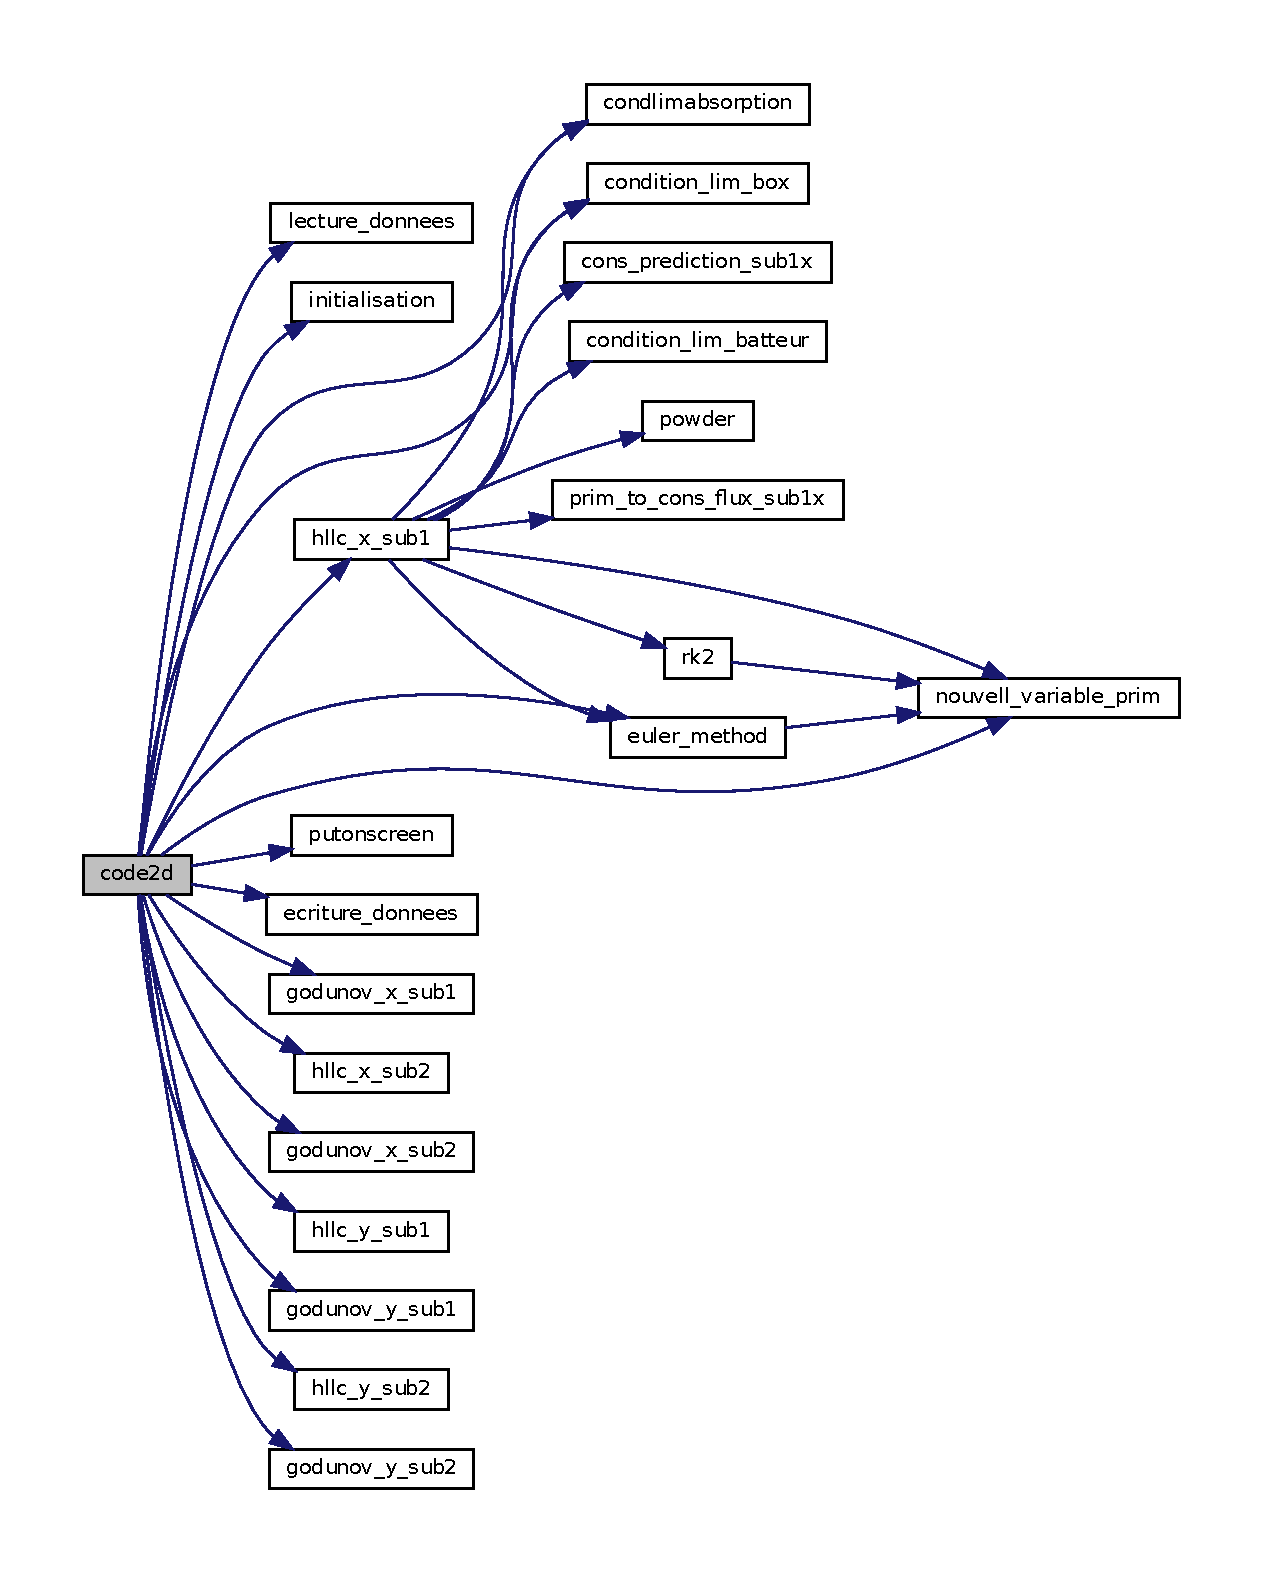
\includegraphics[width=350pt]{main2Dv1_8f90_a8712173bc20143ca5b1b8cbd782b563e_cgraph}
\end{center}
\end{figure}
\mbox{\Hypertarget{main2Dv1_8f90_ae64974281df2d6f2222187665fd79e38}\label{main2Dv1_8f90_ae64974281df2d6f2222187665fd79e38}} 
\index{main2\+Dv1.\+f90@{main2\+Dv1.\+f90}!condition\+\_\+lim\+\_\+batteur@{condition\+\_\+lim\+\_\+batteur}}
\index{condition\+\_\+lim\+\_\+batteur@{condition\+\_\+lim\+\_\+batteur}!main2\+Dv1.\+f90@{main2\+Dv1.\+f90}}
\subsubsection{\texorpdfstring{condition\+\_\+lim\+\_\+batteur()}{condition\_lim\_batteur()}}
{\footnotesize\ttfamily subroutine code2d\+::condition\+\_\+lim\+\_\+batteur (\begin{DoxyParamCaption}\item[{real (kind = dp), dimension(7,0\+:nx+1,0\+:ny+1)}]{Prim,  }\item[{real (kind = dp), dimension(0\+:nx+1,0\+:ny+1)}]{Ein,  }\item[{real (kind = dp), dimension(0\+:nx+1,0\+:ny+1)}]{Pression,  }\item[{real (kind = dp), dimension(0\+:nx+1,0\+:ny+1)}]{S\+O\+U\+N\+D\+\_\+ax,  }\item[{real (kind = dp), dimension(0\+:nx+1,0\+:ny+1)}]{S\+O\+U\+N\+D\+\_\+bx,  }\item[{real (kind = dp), dimension(0\+:nx+1,0\+:ny+1)}]{S\+O\+U\+N\+D\+\_\+ay,  }\item[{real (kind = dp), dimension(0\+:nx+1,0\+:ny+1)}]{S\+O\+U\+N\+D\+\_\+by,  }\item[{real (kind = dp)}]{T\+I\+ME }\end{DoxyParamCaption})}

\mbox{\Hypertarget{main2Dv1_8f90_a2e4131a2a733710c33c03656b6a7fb34}\label{main2Dv1_8f90_a2e4131a2a733710c33c03656b6a7fb34}} 
\index{main2\+Dv1.\+f90@{main2\+Dv1.\+f90}!condition\+\_\+lim\+\_\+box@{condition\+\_\+lim\+\_\+box}}
\index{condition\+\_\+lim\+\_\+box@{condition\+\_\+lim\+\_\+box}!main2\+Dv1.\+f90@{main2\+Dv1.\+f90}}
\subsubsection{\texorpdfstring{condition\+\_\+lim\+\_\+box()}{condition\_lim\_box()}}
{\footnotesize\ttfamily subroutine code2d\+::condition\+\_\+lim\+\_\+box (\begin{DoxyParamCaption}\item[{real (kind = dp), dimension(7,0\+:nx+1,0\+:ny+1)}]{Prim,  }\item[{real (kind = dp), dimension(0\+:nx+1,0\+:ny+1)}]{Ein,  }\item[{real (kind = dp), dimension(0\+:nx+1,0\+:ny+1)}]{Pression,  }\item[{real (kind = dp), dimension(0\+:nx+1,0\+:ny+1)}]{S\+O\+U\+N\+D\+\_\+ax,  }\item[{real (kind = dp), dimension(0\+:nx+1,0\+:ny+1)}]{S\+O\+U\+N\+D\+\_\+bx,  }\item[{real (kind = dp), dimension(0\+:nx+1,0\+:ny+1)}]{S\+O\+U\+N\+D\+\_\+ay,  }\item[{real (kind = dp), dimension(0\+:nx+1,0\+:ny+1)}]{S\+O\+U\+N\+D\+\_\+by }\end{DoxyParamCaption})}

\mbox{\Hypertarget{main2Dv1_8f90_a4fa8d6d2b6084471f67e67e44694e3a7}\label{main2Dv1_8f90_a4fa8d6d2b6084471f67e67e44694e3a7}} 
\index{main2\+Dv1.\+f90@{main2\+Dv1.\+f90}!condlimabsorption@{condlimabsorption}}
\index{condlimabsorption@{condlimabsorption}!main2\+Dv1.\+f90@{main2\+Dv1.\+f90}}
\subsubsection{\texorpdfstring{condlimabsorption()}{condlimabsorption()}}
{\footnotesize\ttfamily subroutine code2d\+::condlimabsorption (\begin{DoxyParamCaption}\item[{real (kind = dp), dimension(nv\+\_\+prim,0\+:nx+1,0\+:ny+1)}]{Prim,  }\item[{real (kind = dp), dimension(0\+:nx+1,0\+:ny+1)}]{Ein,  }\item[{real (kind = dp), dimension(0\+:nx+1,0\+:ny+1)}]{Pression,  }\item[{real (kind = dp), dimension(0\+:nx+1,0\+:ny+1)}]{S\+O\+U\+N\+D\+\_\+ax,  }\item[{real (kind = dp), dimension(0\+:nx+1,0\+:ny+1)}]{S\+O\+U\+N\+D\+\_\+bx,  }\item[{real (kind = dp), dimension(0\+:nx+1,0\+:ny+1)}]{S\+O\+U\+N\+D\+\_\+ay,  }\item[{real (kind = dp), dimension(0\+:nx+1,0\+:ny+1)}]{S\+O\+U\+N\+D\+\_\+by }\end{DoxyParamCaption})}

\mbox{\Hypertarget{main2Dv1_8f90_aff02bfa8466e376e08fed7a99aae4039}\label{main2Dv1_8f90_aff02bfa8466e376e08fed7a99aae4039}} 
\index{main2\+Dv1.\+f90@{main2\+Dv1.\+f90}!ecriture\+\_\+donnees@{ecriture\+\_\+donnees}}
\index{ecriture\+\_\+donnees@{ecriture\+\_\+donnees}!main2\+Dv1.\+f90@{main2\+Dv1.\+f90}}
\subsubsection{\texorpdfstring{ecriture\+\_\+donnees()}{ecriture\_donnees()}}
{\footnotesize\ttfamily subroutine code2d\+::ecriture\+\_\+donnees (\begin{DoxyParamCaption}\item[{real (kind = dp), dimension(1\+:nx)}]{X,  }\item[{real (kind = dp), dimension(1\+:ny)}]{Y,  }\item[{real (kind = dp)}]{Lx,  }\item[{real (kind = dp), dimension(nv\+\_\+prim,0\+:nx+1,0\+:ny+1)}]{Prim,  }\item[{real (kind = dp), dimension(0\+:nx+1,0\+:ny+1)}]{Ein,  }\item[{real (kind = dp), dimension(0\+:nx+1,0\+:ny+1)}]{Pression,  }\item[{real (kind = dp)}]{time,  }\item[{real (kind = dp)}]{DX,  }\item[{real (kind = dp)}]{DY }\end{DoxyParamCaption})}

\mbox{\Hypertarget{main2Dv1_8f90_a1874243fd0ebdb9c1e1cd78468b4cfac}\label{main2Dv1_8f90_a1874243fd0ebdb9c1e1cd78468b4cfac}} 
\index{main2\+Dv1.\+f90@{main2\+Dv1.\+f90}!euler\+\_\+method@{euler\+\_\+method}}
\index{euler\+\_\+method@{euler\+\_\+method}!main2\+Dv1.\+f90@{main2\+Dv1.\+f90}}
\subsubsection{\texorpdfstring{euler\+\_\+method()}{euler\_method()}}
{\footnotesize\ttfamily subroutine code2d\+::euler\+\_\+method (\begin{DoxyParamCaption}\item[{real (kind = dp)}]{DT,  }\item[{real (kind = dp)}]{time,  }\item[{real (kind = dp)}]{Lx,  }\item[{real (kind = dp), dimension(1\+:nx)}]{X,  }\item[{real (kind = dp), dimension(1\+:ny)}]{Y,  }\item[{real (kind = dp), dimension(8,1\+:nx, 1\+:ny)}]{C\+O\+NS,  }\item[{real (kind = dp), dimension(7,0\+:nx+1,0\+:ny+1)}]{Prim,  }\item[{real (kind = dp), dimension(0\+:nx+1,0\+:ny+1)}]{Ein,  }\item[{real (kind = dp), dimension(0\+:nx+1,0\+:ny+1)}]{S\+O\+U\+N\+D\+\_\+ax,  }\item[{real (kind = dp), dimension(0\+:nx+1,0\+:ny+1)}]{S\+O\+U\+N\+D\+\_\+bx,  }\item[{real (kind = dp), dimension(0\+:nx+1,0\+:ny+1)}]{S\+O\+U\+N\+D\+\_\+ay,  }\item[{real (kind = dp), dimension(0\+:nx+1,0\+:ny+1)}]{S\+O\+U\+N\+D\+\_\+by,  }\item[{real (kind = dp), dimension(0\+:nx+1,0\+:ny+1)}]{Pression,  }\item[{integer}]{it }\end{DoxyParamCaption})}

Here is the call graph for this function\+:
\nopagebreak
\begin{figure}[H]
\begin{center}
\leavevmode
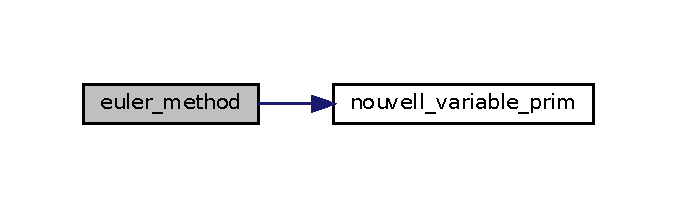
\includegraphics[width=325pt]{main2Dv1_8f90_a1874243fd0ebdb9c1e1cd78468b4cfac_cgraph}
\end{center}
\end{figure}
\mbox{\Hypertarget{main2Dv1_8f90_aec66a1d113ade1d60ad864482ea8e4cf}\label{main2Dv1_8f90_aec66a1d113ade1d60ad864482ea8e4cf}} 
\index{main2\+Dv1.\+f90@{main2\+Dv1.\+f90}!godunov\+\_\+x\+\_\+sub1@{godunov\+\_\+x\+\_\+sub1}}
\index{godunov\+\_\+x\+\_\+sub1@{godunov\+\_\+x\+\_\+sub1}!main2\+Dv1.\+f90@{main2\+Dv1.\+f90}}
\subsubsection{\texorpdfstring{godunov\+\_\+x\+\_\+sub1()}{godunov\_x\_sub1()}}
{\footnotesize\ttfamily subroutine code2d\+::godunov\+\_\+x\+\_\+sub1 (\begin{DoxyParamCaption}\item[{real(kind=dp), dimension(8,1\+:nx,1\+:ny)}]{cons,  }\item[{real(kind=dp), dimension(8,0\+:nx,0\+:ny)}]{flux,  }\item[{real(kind=dp)}]{dt,  }\item[{real(kind=dp)}]{dx }\end{DoxyParamCaption})}

\mbox{\Hypertarget{main2Dv1_8f90_a95998c355563e1e58114aea99de5433b}\label{main2Dv1_8f90_a95998c355563e1e58114aea99de5433b}} 
\index{main2\+Dv1.\+f90@{main2\+Dv1.\+f90}!godunov\+\_\+x\+\_\+sub2@{godunov\+\_\+x\+\_\+sub2}}
\index{godunov\+\_\+x\+\_\+sub2@{godunov\+\_\+x\+\_\+sub2}!main2\+Dv1.\+f90@{main2\+Dv1.\+f90}}
\subsubsection{\texorpdfstring{godunov\+\_\+x\+\_\+sub2()}{godunov\_x\_sub2()}}
{\footnotesize\ttfamily subroutine code2d\+::godunov\+\_\+x\+\_\+sub2 (\begin{DoxyParamCaption}\item[{real(kind=dp), dimension(8,1\+:nx,1\+:ny)}]{cons,  }\item[{real(kind=dp), dimension(8,0\+:nx,0\+:ny)}]{flux,  }\item[{real(kind=dp)}]{dt,  }\item[{real(kind=dp)}]{dx }\end{DoxyParamCaption})}

\mbox{\Hypertarget{main2Dv1_8f90_a99b7b2764471880074ec2cb4448c3232}\label{main2Dv1_8f90_a99b7b2764471880074ec2cb4448c3232}} 
\index{main2\+Dv1.\+f90@{main2\+Dv1.\+f90}!godunov\+\_\+y\+\_\+sub1@{godunov\+\_\+y\+\_\+sub1}}
\index{godunov\+\_\+y\+\_\+sub1@{godunov\+\_\+y\+\_\+sub1}!main2\+Dv1.\+f90@{main2\+Dv1.\+f90}}
\subsubsection{\texorpdfstring{godunov\+\_\+y\+\_\+sub1()}{godunov\_y\_sub1()}}
{\footnotesize\ttfamily subroutine code2d\+::godunov\+\_\+y\+\_\+sub1 (\begin{DoxyParamCaption}\item[{real(kind=dp), dimension(8,1\+:nx,1\+:ny)}]{cons,  }\item[{real(kind=dp), dimension(8,0\+:nx,0\+:ny)}]{flux,  }\item[{real(kind=dp)}]{dt,  }\item[{real(kind=dp)}]{dx }\end{DoxyParamCaption})}

\mbox{\Hypertarget{main2Dv1_8f90_af2bc178b3e046a285b7e624ecb7246b8}\label{main2Dv1_8f90_af2bc178b3e046a285b7e624ecb7246b8}} 
\index{main2\+Dv1.\+f90@{main2\+Dv1.\+f90}!godunov\+\_\+y\+\_\+sub2@{godunov\+\_\+y\+\_\+sub2}}
\index{godunov\+\_\+y\+\_\+sub2@{godunov\+\_\+y\+\_\+sub2}!main2\+Dv1.\+f90@{main2\+Dv1.\+f90}}
\subsubsection{\texorpdfstring{godunov\+\_\+y\+\_\+sub2()}{godunov\_y\_sub2()}}
{\footnotesize\ttfamily subroutine code2d\+::godunov\+\_\+y\+\_\+sub2 (\begin{DoxyParamCaption}\item[{real(kind=dp), dimension(8,1\+:nx,1\+:ny)}]{cons,  }\item[{real(kind=dp), dimension(8,0\+:nx,0\+:ny)}]{flux,  }\item[{real(kind=dp)}]{dt,  }\item[{real(kind=dp)}]{dx }\end{DoxyParamCaption})}

\mbox{\Hypertarget{main2Dv1_8f90_ad651365c868e762b033239f23065b179}\label{main2Dv1_8f90_ad651365c868e762b033239f23065b179}} 
\index{main2\+Dv1.\+f90@{main2\+Dv1.\+f90}!hllc\+\_\+x\+\_\+sub1@{hllc\+\_\+x\+\_\+sub1}}
\index{hllc\+\_\+x\+\_\+sub1@{hllc\+\_\+x\+\_\+sub1}!main2\+Dv1.\+f90@{main2\+Dv1.\+f90}}
\subsubsection{\texorpdfstring{hllc\+\_\+x\+\_\+sub1()}{hllc\_x\_sub1()}}
{\footnotesize\ttfamily subroutine code2d\+::hllc\+\_\+x\+\_\+sub1 (\begin{DoxyParamCaption}\item[{real (kind = dp), dimension(7,0\+:nx+1,0\+:ny+1)}]{prim,  }\item[{real (kind = dp), dimension(8,0\+:nx,0\+:ny)}]{flux }\end{DoxyParamCaption})}

\mbox{\Hypertarget{main2Dv1_8f90_a542b368221e3c5b6eed538ddc6538ca5}\label{main2Dv1_8f90_a542b368221e3c5b6eed538ddc6538ca5}} 
\index{main2\+Dv1.\+f90@{main2\+Dv1.\+f90}!hllc\+\_\+x\+\_\+sub2@{hllc\+\_\+x\+\_\+sub2}}
\index{hllc\+\_\+x\+\_\+sub2@{hllc\+\_\+x\+\_\+sub2}!main2\+Dv1.\+f90@{main2\+Dv1.\+f90}}
\subsubsection{\texorpdfstring{hllc\+\_\+x\+\_\+sub2()}{hllc\_x\_sub2()}}
{\footnotesize\ttfamily subroutine code2d\+::hllc\+\_\+x\+\_\+sub2 (\begin{DoxyParamCaption}\item[{real (kind = dp), dimension(7,0\+:nx+1,0\+:ny+1)}]{prim,  }\item[{real (kind = dp), dimension(8,0\+:nx,0\+:ny)}]{flux }\end{DoxyParamCaption})}

\mbox{\Hypertarget{main2Dv1_8f90_a3abf545225182ebde80c72121d2de6f2}\label{main2Dv1_8f90_a3abf545225182ebde80c72121d2de6f2}} 
\index{main2\+Dv1.\+f90@{main2\+Dv1.\+f90}!hllc\+\_\+y\+\_\+sub1@{hllc\+\_\+y\+\_\+sub1}}
\index{hllc\+\_\+y\+\_\+sub1@{hllc\+\_\+y\+\_\+sub1}!main2\+Dv1.\+f90@{main2\+Dv1.\+f90}}
\subsubsection{\texorpdfstring{hllc\+\_\+y\+\_\+sub1()}{hllc\_y\_sub1()}}
{\footnotesize\ttfamily subroutine code2d\+::hllc\+\_\+y\+\_\+sub1 (\begin{DoxyParamCaption}\item[{real (kind = dp), dimension(7,0\+:nx+1,0\+:ny+1)}]{prim,  }\item[{real (kind = dp), dimension(8,0\+:nx,0\+:ny)}]{flux }\end{DoxyParamCaption})}

\mbox{\Hypertarget{main2Dv1_8f90_a66b4ae2bdd9b70fca9079c3827fa8c30}\label{main2Dv1_8f90_a66b4ae2bdd9b70fca9079c3827fa8c30}} 
\index{main2\+Dv1.\+f90@{main2\+Dv1.\+f90}!hllc\+\_\+y\+\_\+sub2@{hllc\+\_\+y\+\_\+sub2}}
\index{hllc\+\_\+y\+\_\+sub2@{hllc\+\_\+y\+\_\+sub2}!main2\+Dv1.\+f90@{main2\+Dv1.\+f90}}
\subsubsection{\texorpdfstring{hllc\+\_\+y\+\_\+sub2()}{hllc\_y\_sub2()}}
{\footnotesize\ttfamily subroutine code2d\+::hllc\+\_\+y\+\_\+sub2 (\begin{DoxyParamCaption}\item[{real (kind = dp), dimension(7,0\+:nx+1,0\+:ny+1)}]{prim,  }\item[{real (kind = dp), dimension(8,0\+:nx,0\+:ny)}]{flux }\end{DoxyParamCaption})}

\mbox{\Hypertarget{main2Dv1_8f90_afb1c4be5a540eb38b6217aa886b964a5}\label{main2Dv1_8f90_afb1c4be5a540eb38b6217aa886b964a5}} 
\index{main2\+Dv1.\+f90@{main2\+Dv1.\+f90}!initialisation@{initialisation}}
\index{initialisation@{initialisation}!main2\+Dv1.\+f90@{main2\+Dv1.\+f90}}
\subsubsection{\texorpdfstring{initialisation()}{initialisation()}}
{\footnotesize\ttfamily subroutine code2d\+::initialisation (\begin{DoxyParamCaption}\item[{real (kind = dp)}]{DX,  }\item[{real (kind = dp)}]{DY,  }\item[{real (kind = dp), dimension(1\+:nx)}]{X,  }\item[{real (kind = dp), dimension(1\+:ny)}]{Y,  }\item[{real (kind = dp), dimension(nv\+\_\+prim, 0\+:nx+1,0\+:ny+1)}]{Prim,  }\item[{real (kind = dp), dimension(0\+:nx+1,0\+:ny+1)}]{S\+O\+U\+N\+D\+\_\+ax,  }\item[{real (kind = dp), dimension(0\+:nx+1,0\+:ny+1)}]{S\+O\+U\+N\+D\+\_\+bx,  }\item[{real (kind = dp), dimension(0\+:nx+1,0\+:ny+1)}]{S\+O\+U\+N\+D\+\_\+ay,  }\item[{real (kind = dp), dimension(0\+:nx+1,0\+:ny+1)}]{S\+O\+U\+N\+D\+\_\+by,  }\item[{real (kind = dp), dimension(0\+:nx+1,0\+:ny+1)}]{Ein,  }\item[{real (kind = dp), dimension(nv\+\_\+prim+1,1\+:nx,1\+:ny)}]{C\+O\+NS,  }\item[{real (kind = dp), dimension(0\+:nx+1,0\+:ny+1)}]{Pression,  }\item[{real (kind = dp)}]{Lx }\end{DoxyParamCaption})}

\mbox{\Hypertarget{main2Dv1_8f90_a7e06ba833aef7743b6a2f1be79f4bc2e}\label{main2Dv1_8f90_a7e06ba833aef7743b6a2f1be79f4bc2e}} 
\index{main2\+Dv1.\+f90@{main2\+Dv1.\+f90}!lecture\+\_\+donnees@{lecture\+\_\+donnees}}
\index{lecture\+\_\+donnees@{lecture\+\_\+donnees}!main2\+Dv1.\+f90@{main2\+Dv1.\+f90}}
\subsubsection{\texorpdfstring{lecture\+\_\+donnees()}{lecture\_donnees()}}
{\footnotesize\ttfamily subroutine code2d\+::lecture\+\_\+donnees (\begin{DoxyParamCaption}\item[{real (kind = dp)}]{Lx,  }\item[{real (kind = dp)}]{Ly }\end{DoxyParamCaption})}

\mbox{\Hypertarget{main2Dv1_8f90_a7e8756401e9774b000709214edc41a76}\label{main2Dv1_8f90_a7e8756401e9774b000709214edc41a76}} 
\index{main2\+Dv1.\+f90@{main2\+Dv1.\+f90}!nouvell\+\_\+variable\+\_\+prim@{nouvell\+\_\+variable\+\_\+prim}}
\index{nouvell\+\_\+variable\+\_\+prim@{nouvell\+\_\+variable\+\_\+prim}!main2\+Dv1.\+f90@{main2\+Dv1.\+f90}}
\subsubsection{\texorpdfstring{nouvell\+\_\+variable\+\_\+prim()}{nouvell\_variable\_prim()}}
{\footnotesize\ttfamily subroutine code2d\+::nouvell\+\_\+variable\+\_\+prim (\begin{DoxyParamCaption}\item[{real (kind = dp), dimension(7,0\+:nx+1,0\+:ny+1)}]{Prim,  }\item[{real (kind = dp), dimension(0\+:nx+1,0\+:ny+1)}]{Ein,  }\item[{real (kind = dp), dimension(0\+:nx+1,0\+:ny+1)}]{S\+O\+U\+N\+D\+\_\+ax,  }\item[{real (kind = dp), dimension(0\+:nx+1,0\+:ny+1)}]{S\+O\+U\+N\+D\+\_\+bx,  }\item[{real (kind = dp), dimension(0\+:nx+1,0\+:ny+1)}]{S\+O\+U\+N\+D\+\_\+ay,  }\item[{real (kind = dp), dimension(0\+:nx+1,0\+:ny+1)}]{S\+O\+U\+N\+D\+\_\+by,  }\item[{real (kind = dp), dimension(8,1\+:nx,1\+:ny)}]{C\+O\+NS,  }\item[{real (kind = dp), dimension(0\+:nx+1,0\+:ny+1)}]{Pression,  }\item[{integer}]{it }\end{DoxyParamCaption})}

\mbox{\Hypertarget{main2Dv1_8f90_a8a5b072c001df1496416cc96562c9916}\label{main2Dv1_8f90_a8a5b072c001df1496416cc96562c9916}} 
\index{main2\+Dv1.\+f90@{main2\+Dv1.\+f90}!putonscreen@{putonscreen}}
\index{putonscreen@{putonscreen}!main2\+Dv1.\+f90@{main2\+Dv1.\+f90}}
\subsubsection{\texorpdfstring{putonscreen()}{putonscreen()}}
{\footnotesize\ttfamily subroutine code2d\+::putonscreen (\begin{DoxyParamCaption}{ }\end{DoxyParamCaption})}


\hypertarget{mainSW_8f90}{}\section{src/main\+SW.f90 File Reference}
\label{mainSW_8f90}\index{src/main\+S\+W.\+f90@{src/main\+S\+W.\+f90}}
\subsection*{Modules}
\begin{DoxyCompactItemize}
\item 
module \mbox{\hyperlink{namespaceprecisions}{precisions}}
\item 
module \mbox{\hyperlink{namespaceglobalparam}{globalparam}}
\item 
module \mbox{\hyperlink{namespacemodeleinterface}{modeleinterface}}
\end{DoxyCompactItemize}
\subsection*{Functions/\+Subroutines}
\begin{DoxyCompactItemize}
\item 
real(kind=dp) function \mbox{\hyperlink{namespacemodeleinterface_a6b953eda7a6bc3e81e6ae451b273b548}{modeleinterface\+::internalen}} (hm, hp)
\item 
real(kind=dp) function \mbox{\hyperlink{namespacemodeleinterface_ad34088de8c0162343994153e8f34921e}{modeleinterface\+::press}} (h, p11)
\item 
real(kind=dp) function \mbox{\hyperlink{namespacemodeleinterface_a1505c575aa44b45a8509fe827f28bc8d}{modeleinterface\+::sound\+\_\+a\+\_\+x}} (h, p11)
\item 
program \mbox{\hyperlink{mainSW_8f90_a8712173bc20143ca5b1b8cbd782b563e}{code2d}}
\item 
subroutine \mbox{\hyperlink{mainSW_8f90_ad651365c868e762b033239f23065b179}{hllc\+\_\+x\+\_\+sub1}} (prim, flux)
\item 
subroutine \mbox{\hyperlink{mainSW_8f90_aec66a1d113ade1d60ad864482ea8e4cf}{godunov\+\_\+x\+\_\+sub1}} (cons, flux, dt, dx)
\item 
subroutine \mbox{\hyperlink{mainSW_8f90_a8a5b072c001df1496416cc96562c9916}{putonscreen}} ()
\item 
subroutine \mbox{\hyperlink{mainSW_8f90_a71aecccc646b5e5547884fff4f3a4320}{ecriture\+\_\+donnees}} (X, Y, Lx, Prim, Pression, time, DX, DY)
\item 
subroutine \mbox{\hyperlink{mainSW_8f90_a7e06ba833aef7743b6a2f1be79f4bc2e}{lecture\+\_\+donnees}} (Lx, Ly)
\item 
subroutine \mbox{\hyperlink{mainSW_8f90_a58ba3803323d27b63b474b0d71dd80cd}{initialisation}} (DX, DY, X, Y, Prim, S\+O\+U\+N\+D\+\_\+ax, Ein, C\+O\+NS, Pression, Lx)
\item 
subroutine \mbox{\hyperlink{mainSW_8f90_a7645bf861c24416d7be2b579253bb6d4}{nouvell\+\_\+variable\+\_\+prim}} (Prim, S\+O\+U\+N\+D\+\_\+ax, C\+O\+NS, Pression, it)
\item 
subroutine \mbox{\hyperlink{mainSW_8f90_a90165511d1e957b38e88d5aa8e349b60}{condlimabsorption}} (Prim, Pression, S\+O\+U\+N\+D\+\_\+ax)
\item 
subroutine \mbox{\hyperlink{mainSW_8f90_ac38992b213d7b23accbdf96615349ef0}{euler\+\_\+method}} (DT, time, Lx, X, Y, C\+O\+NS, Prim, S\+O\+U\+N\+D\+\_\+ax, Pression, it)
\end{DoxyCompactItemize}


\subsection{Function/\+Subroutine Documentation}
\mbox{\Hypertarget{mainSW_8f90_a8712173bc20143ca5b1b8cbd782b563e}\label{mainSW_8f90_a8712173bc20143ca5b1b8cbd782b563e}} 
\index{main\+S\+W.\+f90@{main\+S\+W.\+f90}!code2d@{code2d}}
\index{code2d@{code2d}!main\+S\+W.\+f90@{main\+S\+W.\+f90}}
\subsubsection{\texorpdfstring{code2d()}{code2d()}}
{\footnotesize\ttfamily program code2d (\begin{DoxyParamCaption}{ }\end{DoxyParamCaption})}

Here is the call graph for this function\+:
\nopagebreak
\begin{figure}[H]
\begin{center}
\leavevmode
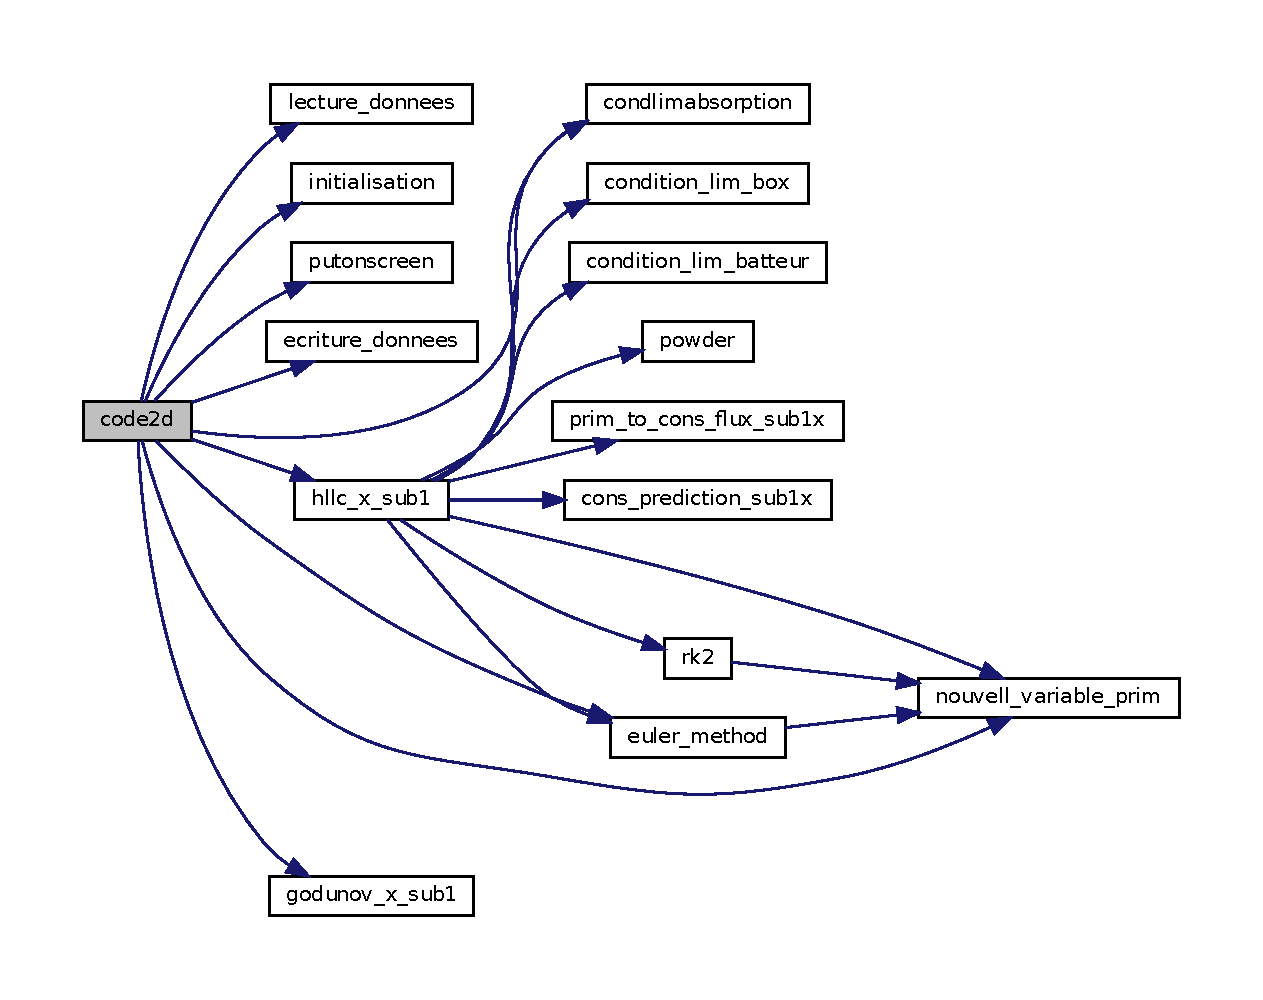
\includegraphics[width=350pt]{mainSW_8f90_a8712173bc20143ca5b1b8cbd782b563e_cgraph}
\end{center}
\end{figure}
\mbox{\Hypertarget{mainSW_8f90_a90165511d1e957b38e88d5aa8e349b60}\label{mainSW_8f90_a90165511d1e957b38e88d5aa8e349b60}} 
\index{main\+S\+W.\+f90@{main\+S\+W.\+f90}!condlimabsorption@{condlimabsorption}}
\index{condlimabsorption@{condlimabsorption}!main\+S\+W.\+f90@{main\+S\+W.\+f90}}
\subsubsection{\texorpdfstring{condlimabsorption()}{condlimabsorption()}}
{\footnotesize\ttfamily subroutine code2d\+::condlimabsorption (\begin{DoxyParamCaption}\item[{real (kind = dp), dimension(nv\+\_\+prim,0\+:nx+1,0\+:ny+1)}]{Prim,  }\item[{real (kind = dp), dimension(0\+:nx+1,0\+:ny+1)}]{Pression,  }\item[{real (kind = dp), dimension(0\+:nx+1,0\+:ny+1)}]{S\+O\+U\+N\+D\+\_\+ax }\end{DoxyParamCaption})}

\mbox{\Hypertarget{mainSW_8f90_a71aecccc646b5e5547884fff4f3a4320}\label{mainSW_8f90_a71aecccc646b5e5547884fff4f3a4320}} 
\index{main\+S\+W.\+f90@{main\+S\+W.\+f90}!ecriture\+\_\+donnees@{ecriture\+\_\+donnees}}
\index{ecriture\+\_\+donnees@{ecriture\+\_\+donnees}!main\+S\+W.\+f90@{main\+S\+W.\+f90}}
\subsubsection{\texorpdfstring{ecriture\+\_\+donnees()}{ecriture\_donnees()}}
{\footnotesize\ttfamily subroutine code2d\+::ecriture\+\_\+donnees (\begin{DoxyParamCaption}\item[{real (kind = dp), dimension(1\+:nx)}]{X,  }\item[{real (kind = dp), dimension(1\+:ny)}]{Y,  }\item[{real (kind = dp)}]{Lx,  }\item[{real (kind = dp), dimension(nv\+\_\+prim,0\+:nx+1,0\+:ny+1)}]{Prim,  }\item[{real (kind = dp), dimension(0\+:nx+1,0\+:ny+1)}]{Pression,  }\item[{real (kind = dp)}]{time,  }\item[{real (kind = dp)}]{DX,  }\item[{real (kind = dp)}]{DY }\end{DoxyParamCaption})}

\mbox{\Hypertarget{mainSW_8f90_ac38992b213d7b23accbdf96615349ef0}\label{mainSW_8f90_ac38992b213d7b23accbdf96615349ef0}} 
\index{main\+S\+W.\+f90@{main\+S\+W.\+f90}!euler\+\_\+method@{euler\+\_\+method}}
\index{euler\+\_\+method@{euler\+\_\+method}!main\+S\+W.\+f90@{main\+S\+W.\+f90}}
\subsubsection{\texorpdfstring{euler\+\_\+method()}{euler\_method()}}
{\footnotesize\ttfamily subroutine code2d\+::euler\+\_\+method (\begin{DoxyParamCaption}\item[{real (kind = dp)}]{DT,  }\item[{real (kind = dp)}]{time,  }\item[{real (kind = dp)}]{Lx,  }\item[{real (kind = dp), dimension(1\+:nx)}]{X,  }\item[{real (kind = dp), dimension(1\+:ny)}]{Y,  }\item[{real (kind = dp), dimension(nv\+\_\+prim,1\+:nx, 1\+:ny)}]{C\+O\+NS,  }\item[{real (kind = dp), dimension(nv\+\_\+prim,0\+:nx+1,0\+:ny+1)}]{Prim,  }\item[{real (kind = dp), dimension(0\+:nx+1,0\+:ny+1)}]{S\+O\+U\+N\+D\+\_\+ax,  }\item[{real (kind = dp), dimension(0\+:nx+1,0\+:ny+1)}]{Pression,  }\item[{integer}]{it }\end{DoxyParamCaption})}

\mbox{\Hypertarget{mainSW_8f90_aec66a1d113ade1d60ad864482ea8e4cf}\label{mainSW_8f90_aec66a1d113ade1d60ad864482ea8e4cf}} 
\index{main\+S\+W.\+f90@{main\+S\+W.\+f90}!godunov\+\_\+x\+\_\+sub1@{godunov\+\_\+x\+\_\+sub1}}
\index{godunov\+\_\+x\+\_\+sub1@{godunov\+\_\+x\+\_\+sub1}!main\+S\+W.\+f90@{main\+S\+W.\+f90}}
\subsubsection{\texorpdfstring{godunov\+\_\+x\+\_\+sub1()}{godunov\_x\_sub1()}}
{\footnotesize\ttfamily subroutine code2d\+::godunov\+\_\+x\+\_\+sub1 (\begin{DoxyParamCaption}\item[{real(kind=dp), dimension(nv\+\_\+prim,1\+:nx,1\+:ny)}]{cons,  }\item[{real(kind=dp), dimension(nv\+\_\+prim,0\+:nx,0\+:ny)}]{flux,  }\item[{real(kind=dp)}]{dt,  }\item[{real(kind=dp)}]{dx }\end{DoxyParamCaption})}

\mbox{\Hypertarget{mainSW_8f90_ad651365c868e762b033239f23065b179}\label{mainSW_8f90_ad651365c868e762b033239f23065b179}} 
\index{main\+S\+W.\+f90@{main\+S\+W.\+f90}!hllc\+\_\+x\+\_\+sub1@{hllc\+\_\+x\+\_\+sub1}}
\index{hllc\+\_\+x\+\_\+sub1@{hllc\+\_\+x\+\_\+sub1}!main\+S\+W.\+f90@{main\+S\+W.\+f90}}
\subsubsection{\texorpdfstring{hllc\+\_\+x\+\_\+sub1()}{hllc\_x\_sub1()}}
{\footnotesize\ttfamily subroutine code2d\+::hllc\+\_\+x\+\_\+sub1 (\begin{DoxyParamCaption}\item[{real (kind = dp), dimension(nv\+\_\+prim,0\+:nx+1,0\+:ny+1)}]{prim,  }\item[{real (kind = dp), dimension(nv\+\_\+prim,0\+:nx,0\+:ny)}]{flux }\end{DoxyParamCaption})}

\mbox{\Hypertarget{mainSW_8f90_a58ba3803323d27b63b474b0d71dd80cd}\label{mainSW_8f90_a58ba3803323d27b63b474b0d71dd80cd}} 
\index{main\+S\+W.\+f90@{main\+S\+W.\+f90}!initialisation@{initialisation}}
\index{initialisation@{initialisation}!main\+S\+W.\+f90@{main\+S\+W.\+f90}}
\subsubsection{\texorpdfstring{initialisation()}{initialisation()}}
{\footnotesize\ttfamily subroutine code2d\+::initialisation (\begin{DoxyParamCaption}\item[{real (kind = dp)}]{DX,  }\item[{real (kind = dp)}]{DY,  }\item[{real (kind = dp), dimension(1\+:nx)}]{X,  }\item[{real (kind = dp), dimension(1\+:ny)}]{Y,  }\item[{real (kind = dp), dimension(nv\+\_\+prim, 0\+:nx+1,0\+:ny+1)}]{Prim,  }\item[{real (kind = dp), dimension(0\+:nx+1,0\+:ny+1)}]{S\+O\+U\+N\+D\+\_\+ax,  }\item[{real (kind = dp), dimension(0\+:nx+1,0\+:ny+1)}]{Ein,  }\item[{real (kind = dp), dimension(nv\+\_\+prim,1\+:nx,1\+:ny)}]{C\+O\+NS,  }\item[{real (kind = dp), dimension(0\+:nx+1,0\+:ny+1)}]{Pression,  }\item[{real (kind = dp)}]{Lx }\end{DoxyParamCaption})}

\mbox{\Hypertarget{mainSW_8f90_a7e06ba833aef7743b6a2f1be79f4bc2e}\label{mainSW_8f90_a7e06ba833aef7743b6a2f1be79f4bc2e}} 
\index{main\+S\+W.\+f90@{main\+S\+W.\+f90}!lecture\+\_\+donnees@{lecture\+\_\+donnees}}
\index{lecture\+\_\+donnees@{lecture\+\_\+donnees}!main\+S\+W.\+f90@{main\+S\+W.\+f90}}
\subsubsection{\texorpdfstring{lecture\+\_\+donnees()}{lecture\_donnees()}}
{\footnotesize\ttfamily subroutine code2d\+::lecture\+\_\+donnees (\begin{DoxyParamCaption}\item[{real (kind = dp)}]{Lx,  }\item[{real (kind = dp)}]{Ly }\end{DoxyParamCaption})}

\mbox{\Hypertarget{mainSW_8f90_a7645bf861c24416d7be2b579253bb6d4}\label{mainSW_8f90_a7645bf861c24416d7be2b579253bb6d4}} 
\index{main\+S\+W.\+f90@{main\+S\+W.\+f90}!nouvell\+\_\+variable\+\_\+prim@{nouvell\+\_\+variable\+\_\+prim}}
\index{nouvell\+\_\+variable\+\_\+prim@{nouvell\+\_\+variable\+\_\+prim}!main\+S\+W.\+f90@{main\+S\+W.\+f90}}
\subsubsection{\texorpdfstring{nouvell\+\_\+variable\+\_\+prim()}{nouvell\_variable\_prim()}}
{\footnotesize\ttfamily subroutine code2d\+::nouvell\+\_\+variable\+\_\+prim (\begin{DoxyParamCaption}\item[{real (kind = dp), dimension(nv\+\_\+prim,0\+:nx+1,0\+:ny+1)}]{Prim,  }\item[{real (kind = dp), dimension(0\+:nx+1,0\+:ny+1)}]{S\+O\+U\+N\+D\+\_\+ax,  }\item[{real (kind = dp), dimension(nv\+\_\+prim,1\+:nx,1\+:ny)}]{C\+O\+NS,  }\item[{real (kind = dp), dimension(0\+:nx+1,0\+:ny+1)}]{Pression,  }\item[{integer}]{it }\end{DoxyParamCaption})}

\mbox{\Hypertarget{mainSW_8f90_a8a5b072c001df1496416cc96562c9916}\label{mainSW_8f90_a8a5b072c001df1496416cc96562c9916}} 
\index{main\+S\+W.\+f90@{main\+S\+W.\+f90}!putonscreen@{putonscreen}}
\index{putonscreen@{putonscreen}!main\+S\+W.\+f90@{main\+S\+W.\+f90}}
\subsubsection{\texorpdfstring{putonscreen()}{putonscreen()}}
{\footnotesize\ttfamily subroutine code2d\+::putonscreen (\begin{DoxyParamCaption}{ }\end{DoxyParamCaption})}


\hypertarget{readXSL_8f90}{}\section{src/read\+X\+SL.f90 File Reference}
\label{readXSL_8f90}\index{src/read\+X\+S\+L.\+f90@{src/read\+X\+S\+L.\+f90}}
\subsection*{Modules}
\begin{DoxyCompactItemize}
\item 
module \mbox{\hyperlink{namespaceprecisions}{precisions}}
\end{DoxyCompactItemize}
\subsection*{Functions/\+Subroutines}
\begin{DoxyCompactItemize}
\item 
program \mbox{\hyperlink{readXSL_8f90_a3972b22411c7969313c9a6e2dd059cc6}{read\+\_\+rewrite}}
\end{DoxyCompactItemize}


\subsection{Function/\+Subroutine Documentation}
\mbox{\Hypertarget{readXSL_8f90_a3972b22411c7969313c9a6e2dd059cc6}\label{readXSL_8f90_a3972b22411c7969313c9a6e2dd059cc6}} 
\index{read\+X\+S\+L.\+f90@{read\+X\+S\+L.\+f90}!read\+\_\+rewrite@{read\+\_\+rewrite}}
\index{read\+\_\+rewrite@{read\+\_\+rewrite}!read\+X\+S\+L.\+f90@{read\+X\+S\+L.\+f90}}
\subsubsection{\texorpdfstring{read\+\_\+rewrite()}{read\_rewrite()}}
{\footnotesize\ttfamily program read\+\_\+rewrite (\begin{DoxyParamCaption}{ }\end{DoxyParamCaption})}


%--- End generated contents ---

% Index
\backmatter
\newpage
\phantomsection
\clearemptydoublepage
\addcontentsline{toc}{chapter}{Index}
\printindex

\end{document}
